\chapter{Experiment Results}
\newpage
\section{Experiment 1}
\label{sec:A_Exp1}
		\begin{figure}[H]
			\centering
		    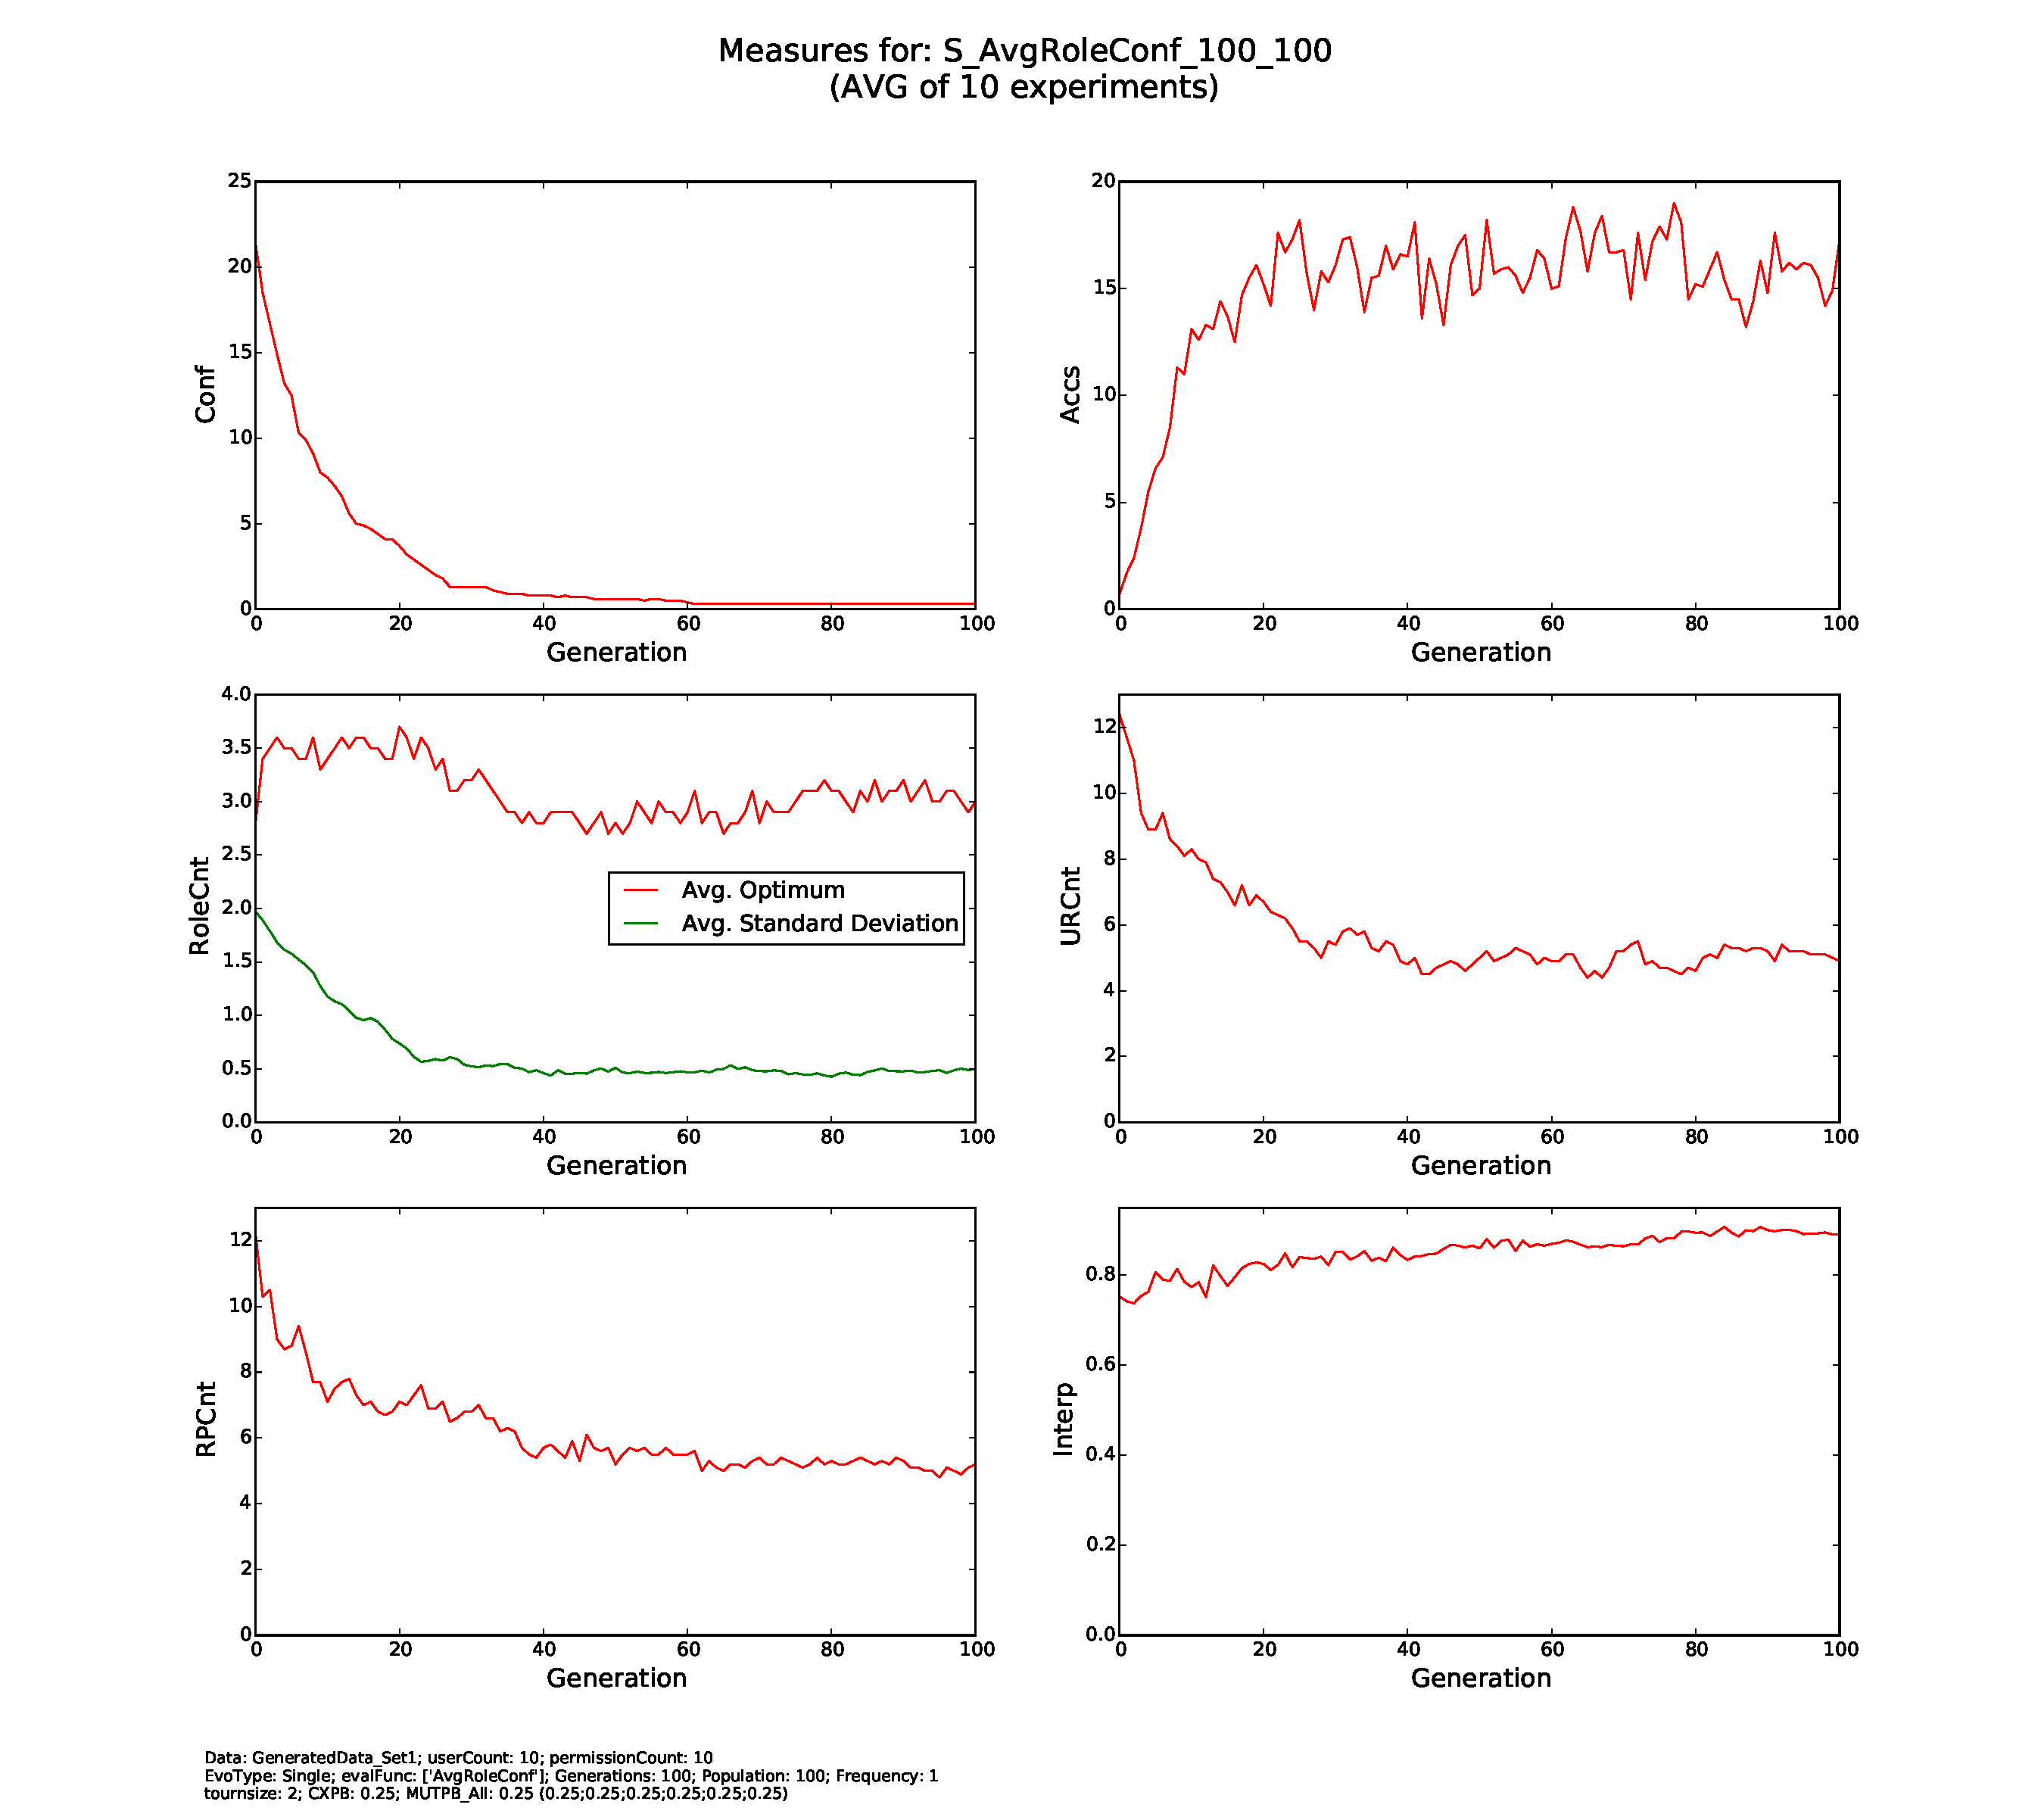
\includegraphics[scale=0.33, trim=4cm 2cm 4cm 0cm, clip=true]{exp1_avgConf}
		    \caption{EXPERIMENT 1c: Results of EvoRoleMiner with Fitness function $F=avg(G_{conf})$ on synthetic dataset 1 with setup in table \ref{tab:setup1}. From u.l. to l.r.: Confidentiality Violations, Availability Violations, Role Count, User-Role Assignments, Role-Permission Assignments, Interpretability.}
		    \label{fig:exp1_avgConf}
		\end{figure}
		
		\begin{figure}[H]
			\centering
		    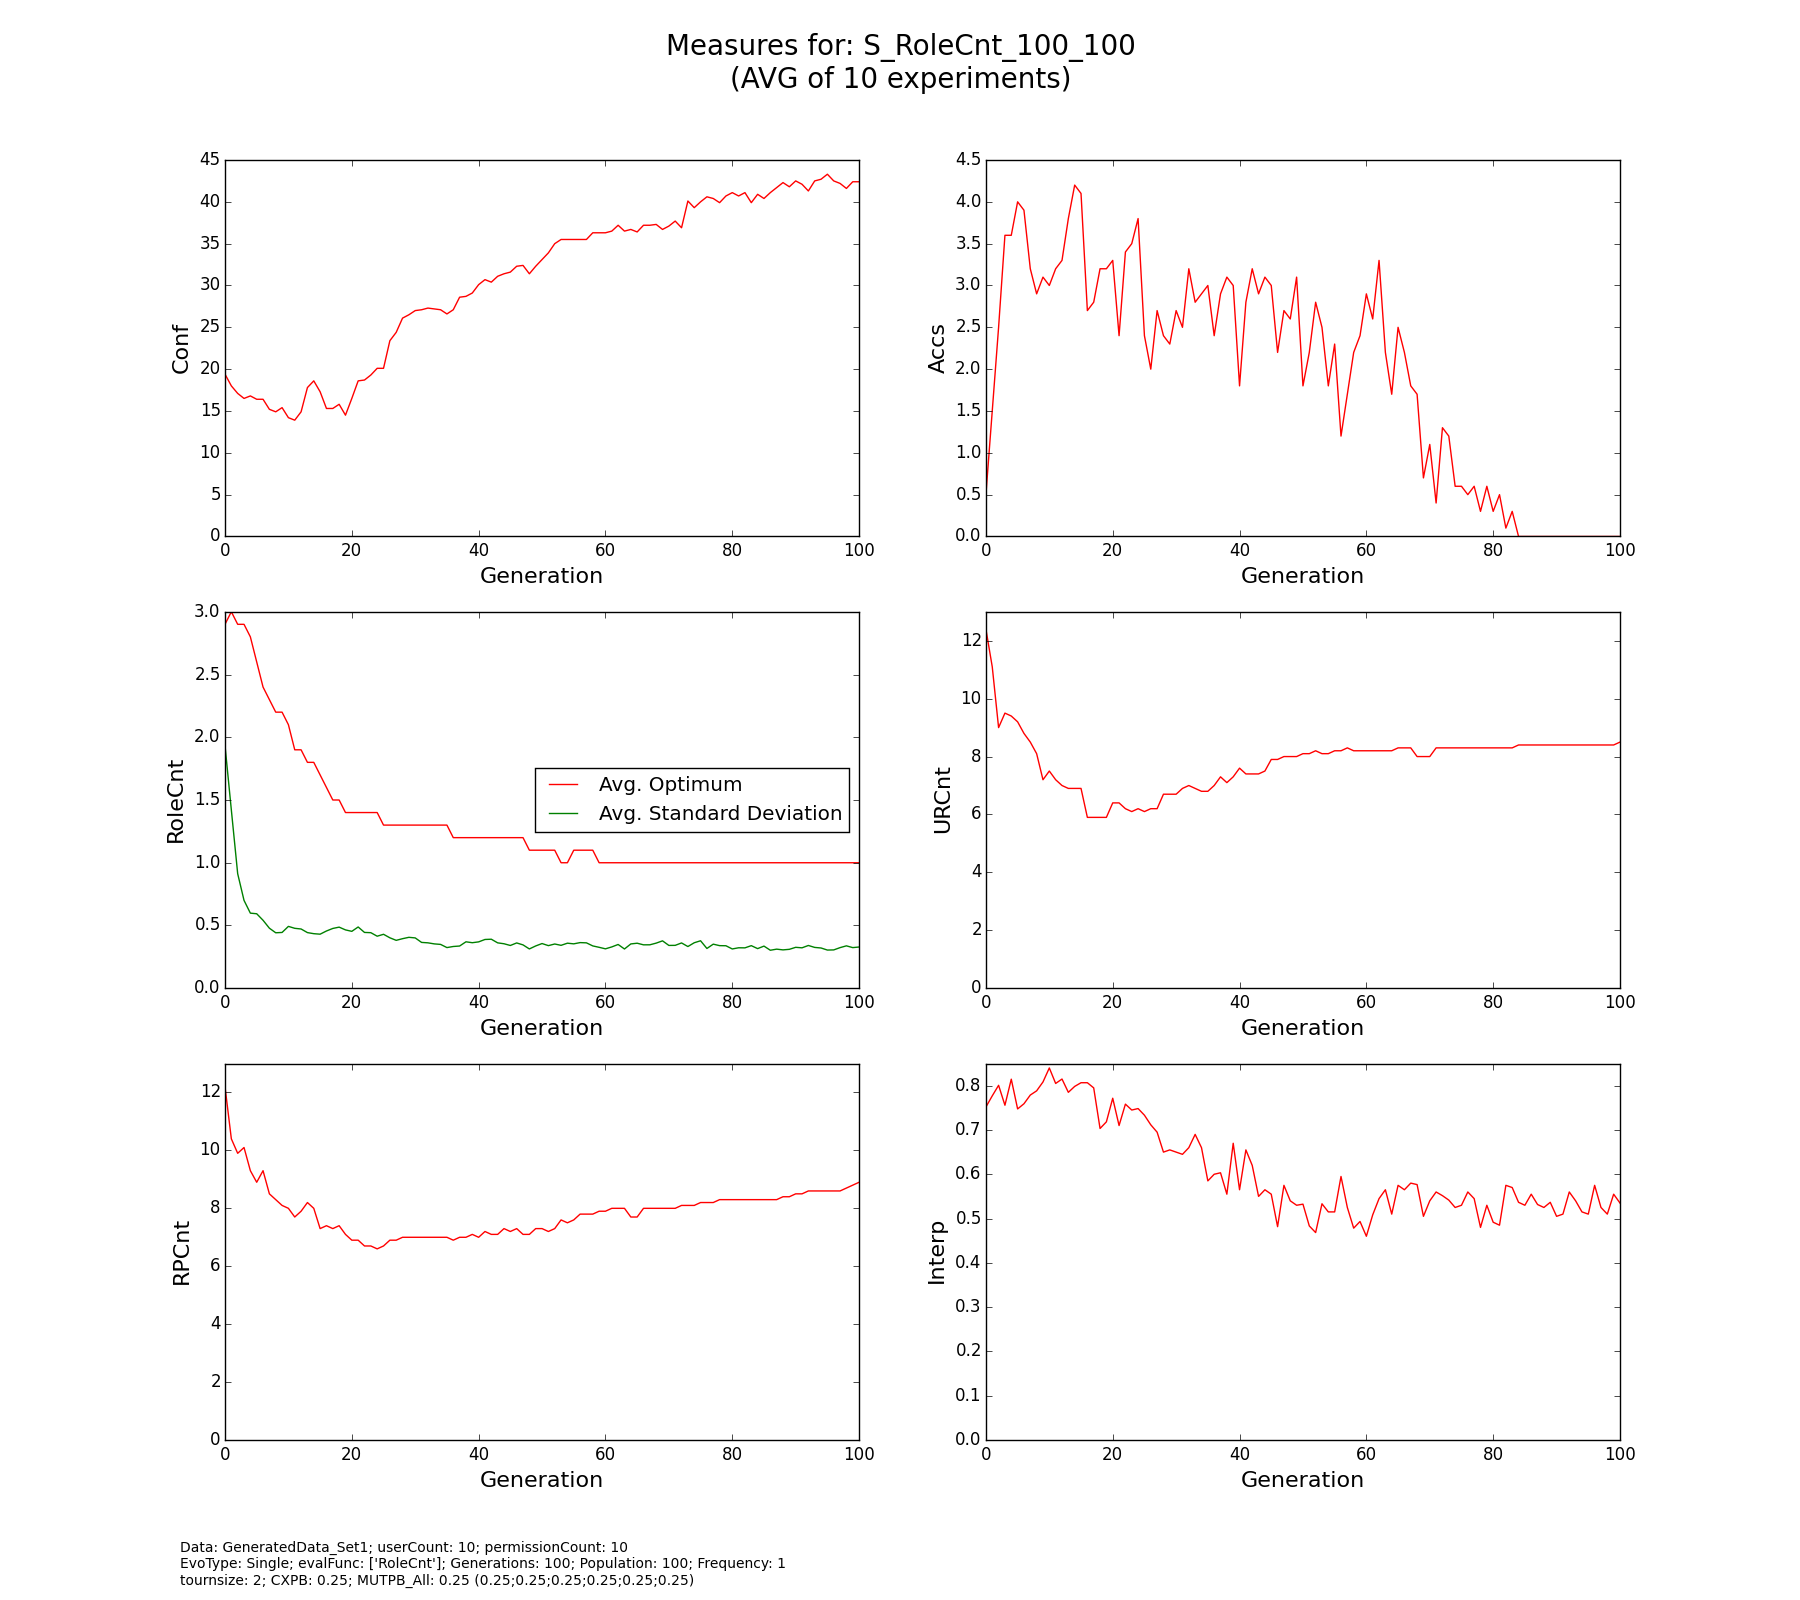
\includegraphics[scale=0.33, trim=4cm 2cm 4cm 0cm, clip=true]{exp1_roleCnt}
		    \caption{EXPERIMENT 1d: Results of EvoRoleMiner with Fitness function $F=|R|$ on synthetic dataset 1 with setup in table \ref{tab:setup1}. From u.l. to l.r.: Confidentiality Violations, Availability Violations, Role Count, User-Role Assignments, Role-Permission Assignments, Interpretability.}
		    \label{fig:exp1_roleCnt}
		\end{figure}
		
		\begin{figure}[H]
			\centering
		    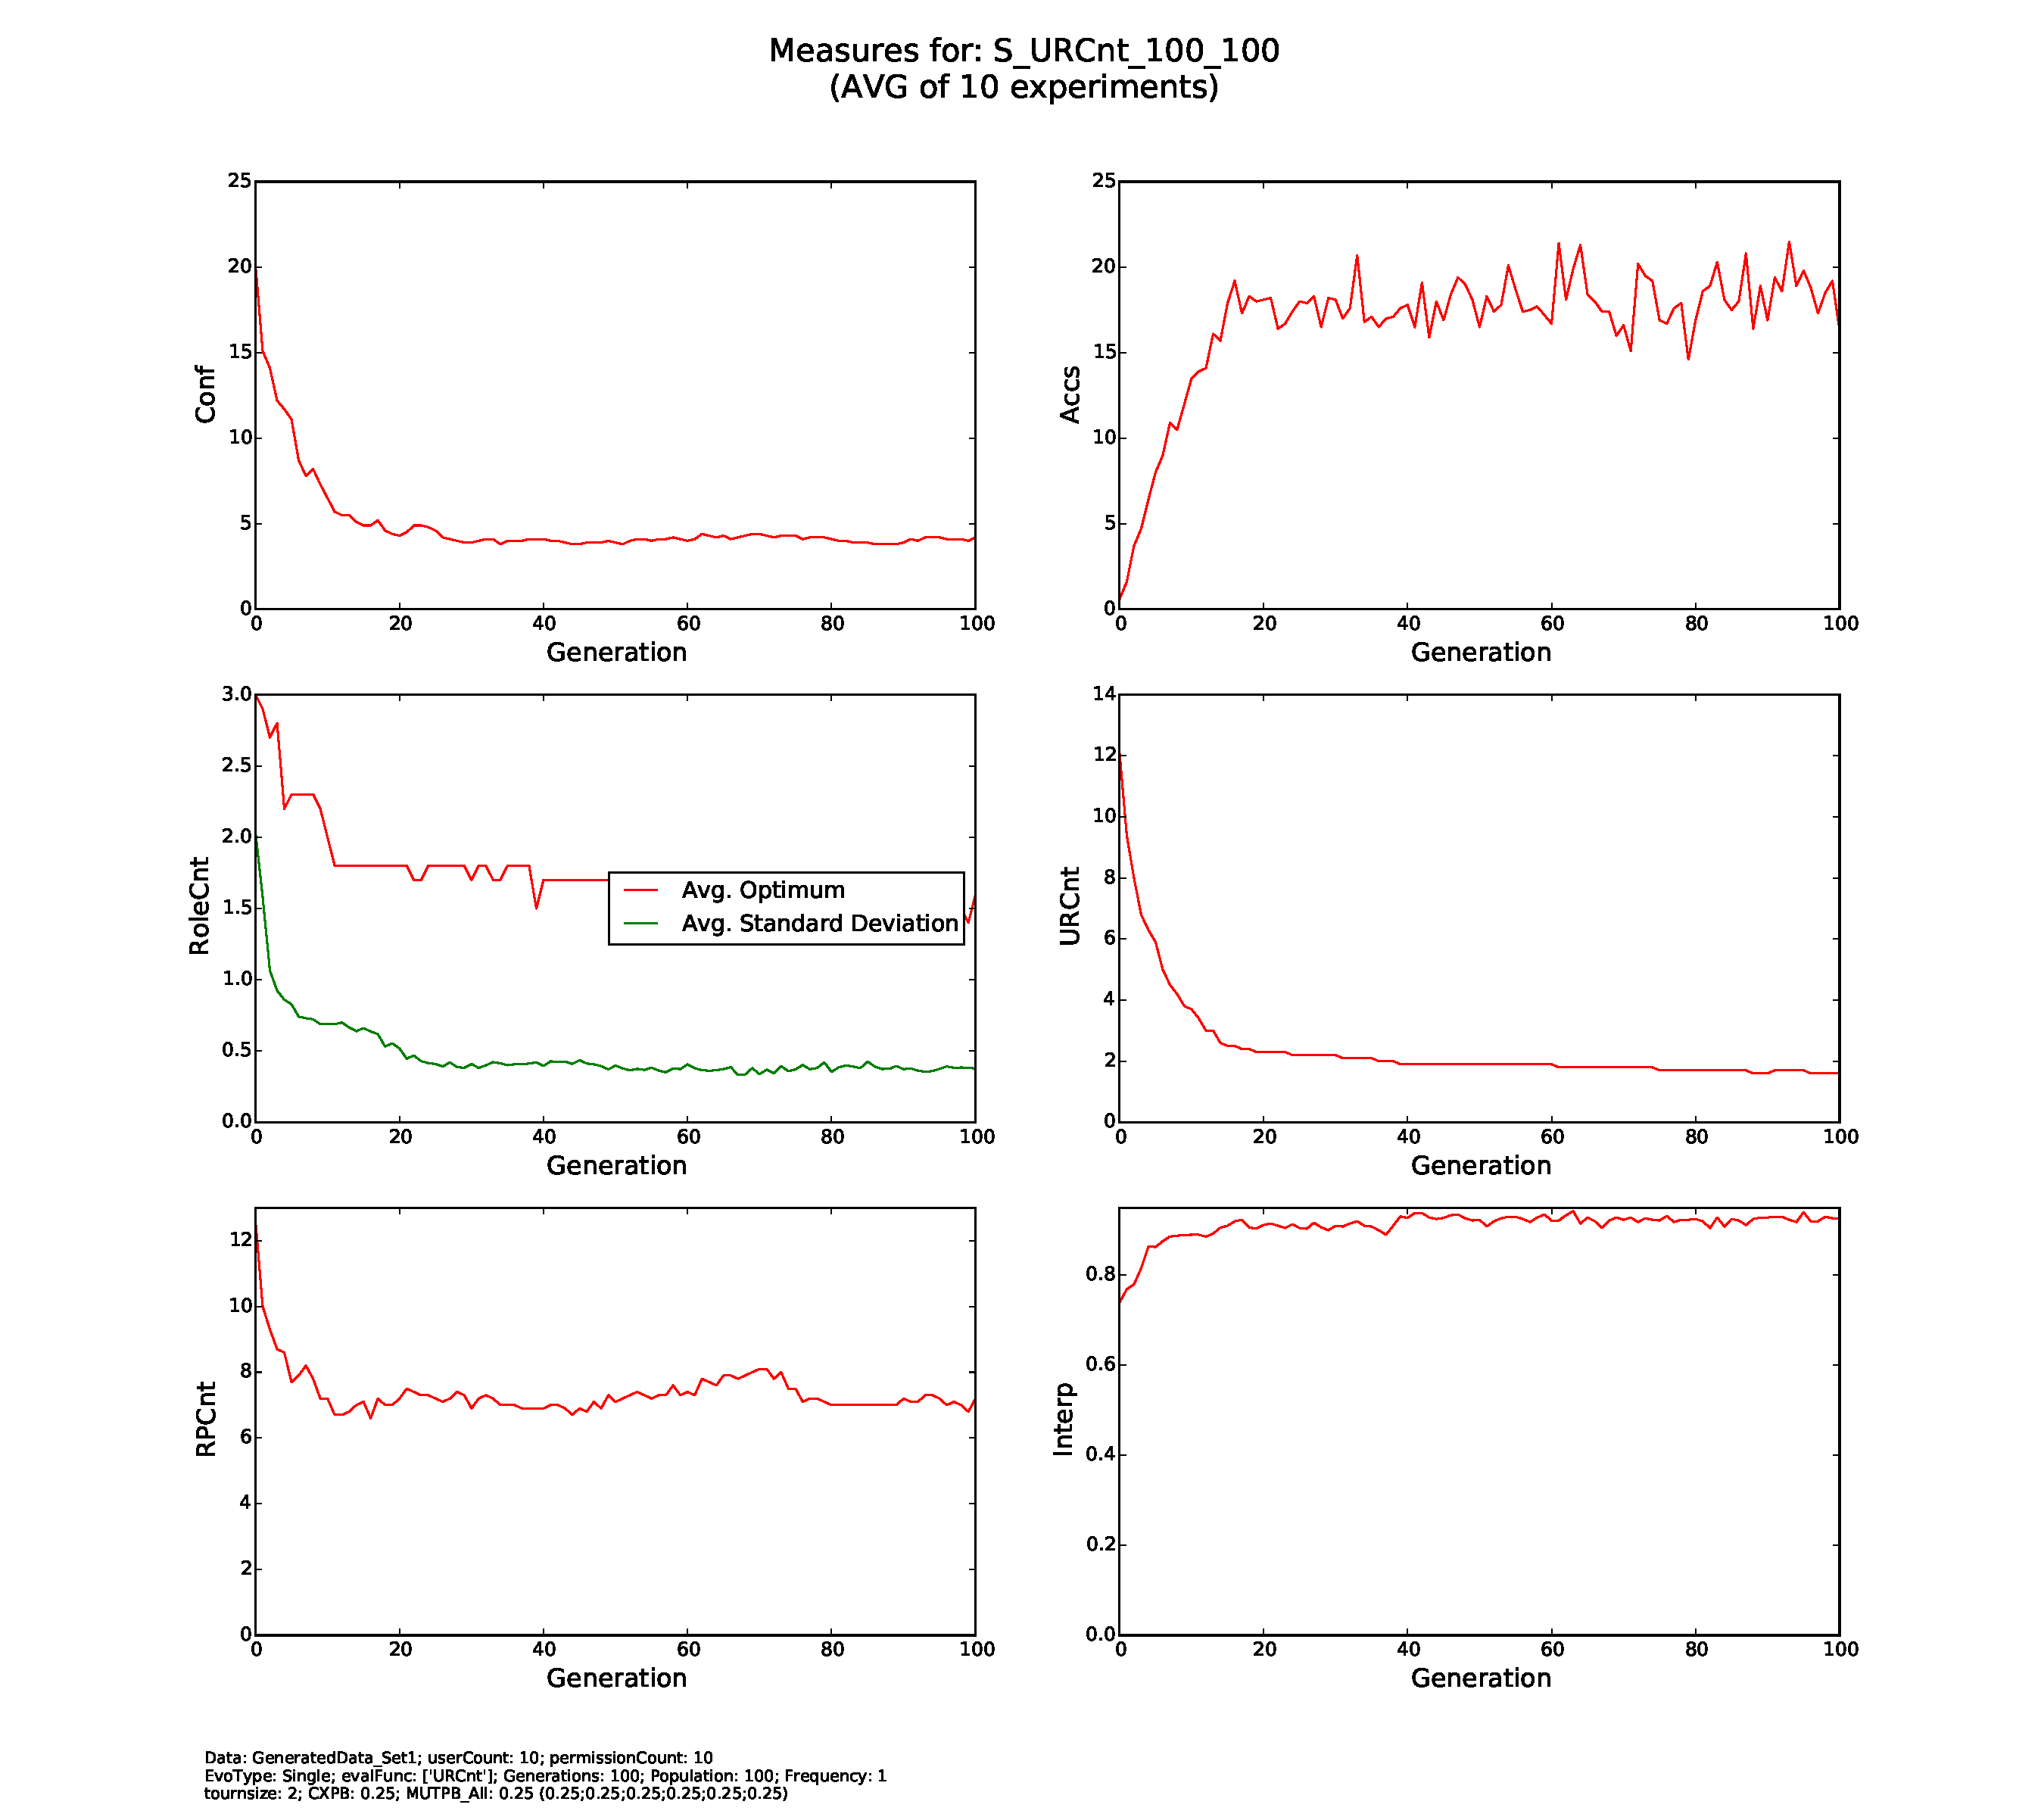
\includegraphics[scale=0.33, trim=4cm 2cm 4cm 0cm, clip=true]{exp1_urCnt}
		    \caption{EXPERIMENT 1e: Results of EvoRoleMiner with Fitness function $F=|UA|$ on synthetic dataset 1 with setup in table \ref{tab:exp1_setup}. From u.l. to l.r.: Confidentiality Violations, Availability Violations, Role Count, User-Role Assignments, Role-Permission Assignments, Interpretability.}
		    \label{fig:exp1_urCnt}
		\end{figure}
		
		\begin{figure}[H]
		    \centering
		    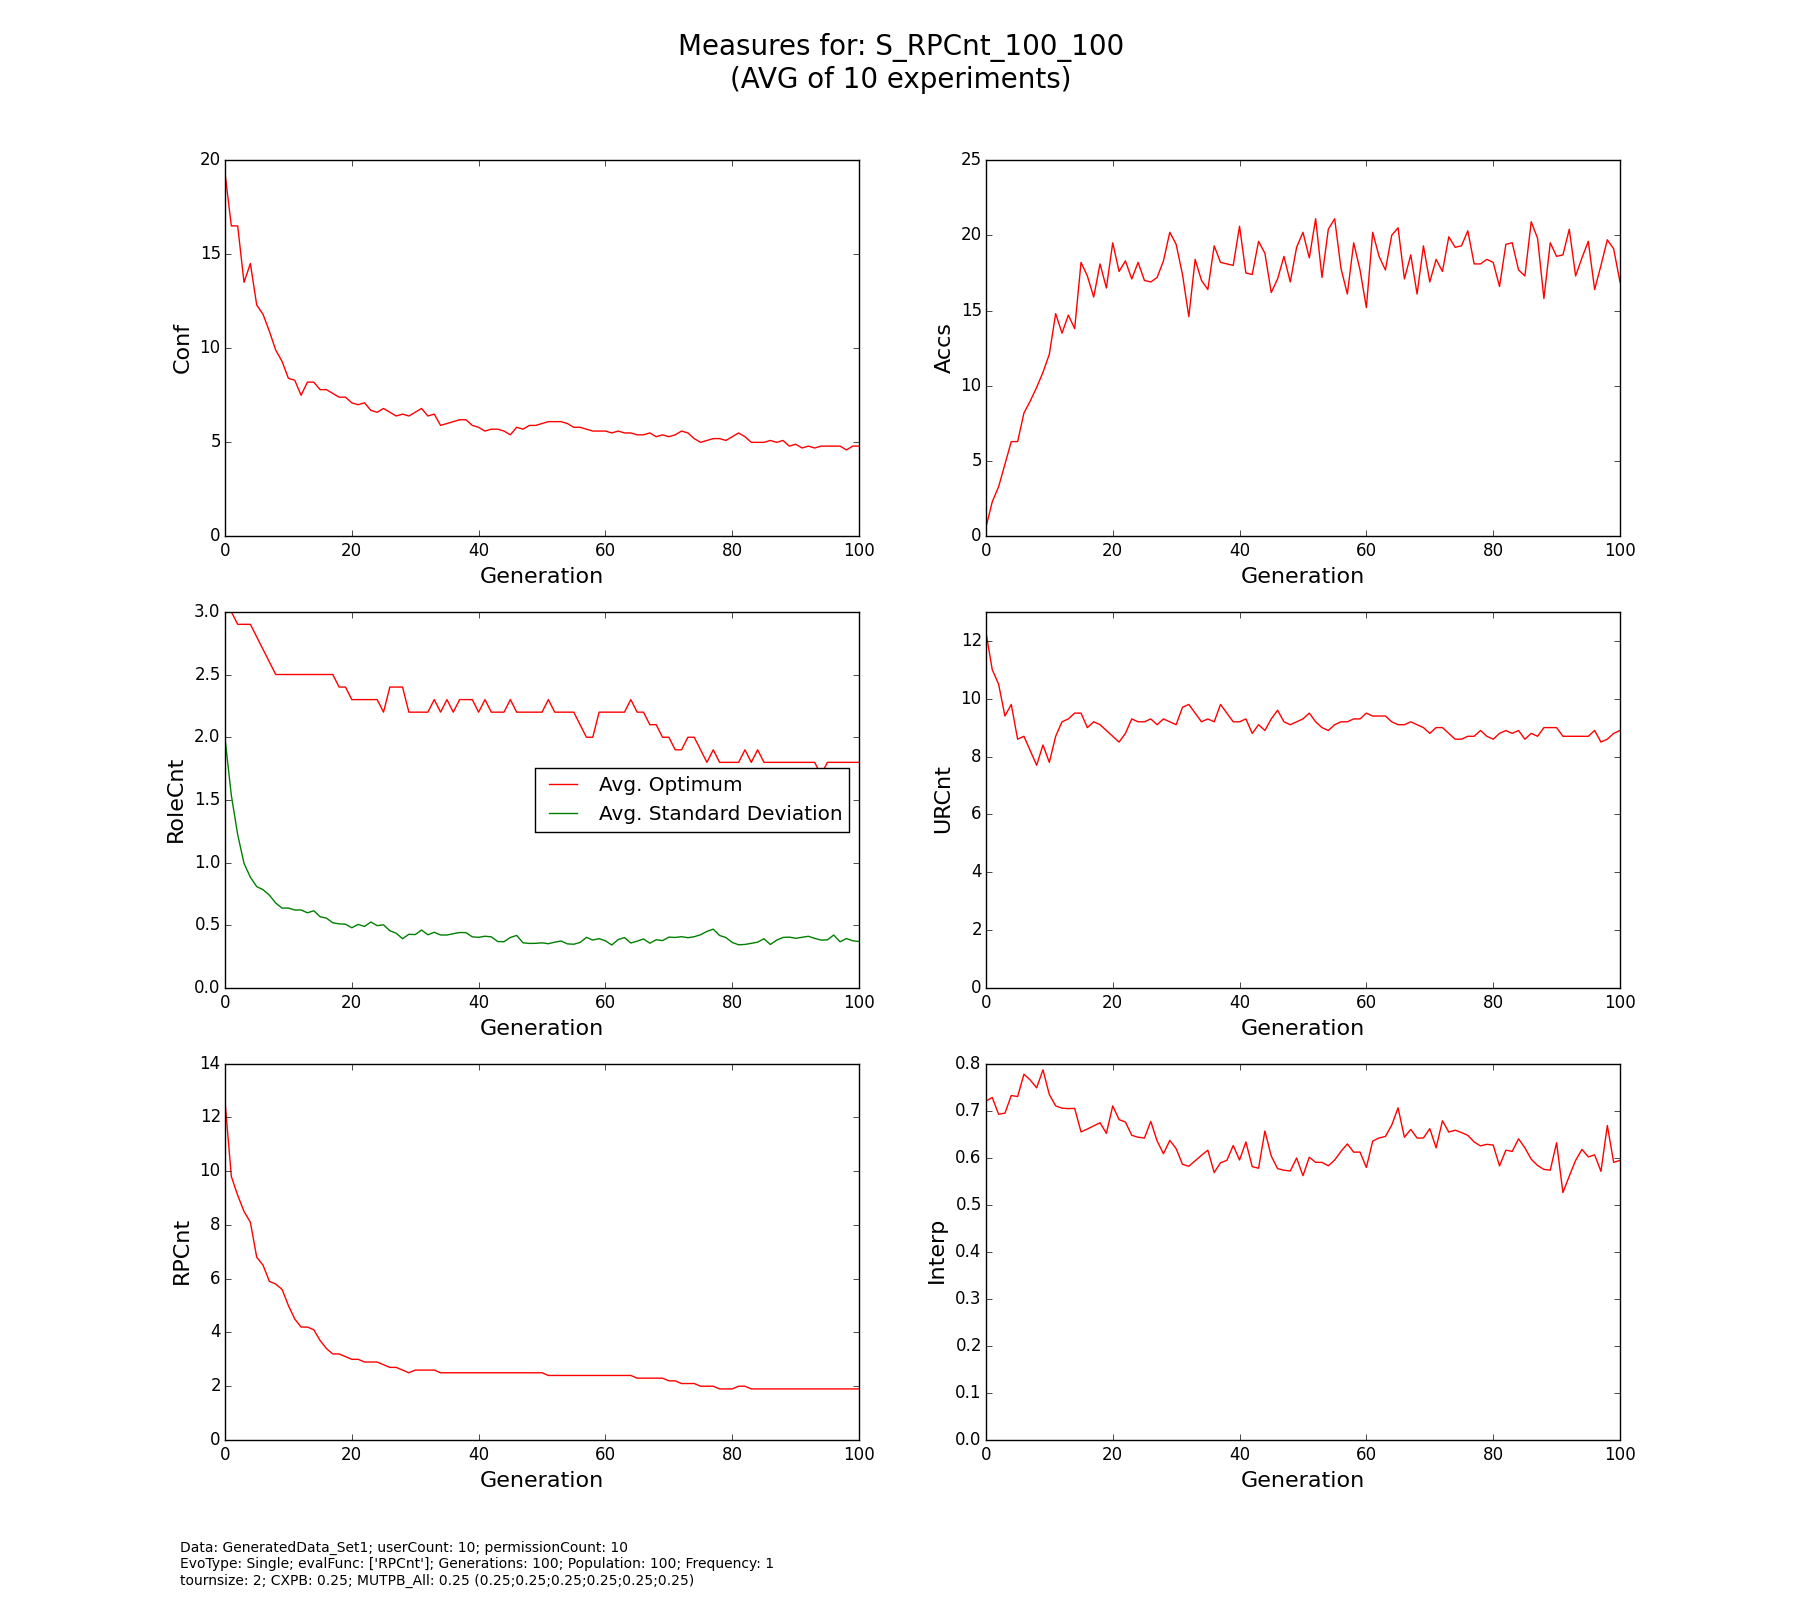
\includegraphics[scale=0.33, trim=4cm 2cm 4cm 0cm, clip=true]{exp1_rpCnt}
	    	\caption{EXPERIMENT 1f: Results of EvoRoleMiner with Fitness function $F=|PA|$ on synthetic dataset 1 with setup in table \ref{tab:exp1_setup}. From u.l. to l.r.: Confidentiality Violations, Availability Violations, Role Count, User-Role Assignments, Role-Permission Assignments, Interpretability.}
	    	\label{fig:exp1_rpCnt}
	    \end{figure}
	
\section{Experiment 2}
\label{sec:A_Exp2}
	\begin{table}[H]
		\centering
		\caption{Evo-RoleMiner: Results of ten experiments for Dataset1 and Healthcare dataset. The values for Fitness, Confidentiality violations ($|G_{conf}|$), Availability violations ($|G_{accs}|$), Roles ($|R|$), User-Role-Assignments ($|UA|$) and Role-Permission assignments ($|PA|$) are the average minimum in the last Generation of all experiments. The values for Interpretability (INT) are the average maximum in the last Generation of all experiments. The time is the average runtime in seconds of all experiments.}
		\label{tab:exp2_results}
		\subcaption*{DATASET1}
		\begin{adjustbox}{width=\textwidth}
			\begin{tabular}{|l|l|c|c|c|c|c|c|c|c|}
				\hline
				\rowcolor{myGray} 
				\textbf{Experiment} & \textbf{Fitness Function} & \textbf{Fitness} & \textbf{$|G_{conf}|$} & \textbf{$|G_{accs}|$} & \textbf{$|R|$} & \textbf{$|UA|$} & \textbf{$|PA|$} & \textbf{INT} & \textbf{Time (in sec)}\\ \hline
				2a & $F_{basic}^{min}$ &   0.38   &   2.8   &   0   &   2   &   8.9   &   7.9   &  1   &   336\\ \hline
				2b & $F_{edge}^{min}$ &    0.15    &   2.8   &   0   &   3.1   &   9.6   &   11.1   &   1   &   343\\ \hline 
			\end{tabular}
		\end{adjustbox}
		\bigskip
		\subcaption*{HEALTHCARE DATASET}
		\begin{adjustbox}{width=\textwidth}
			\begin{tabular}{|l|l|c|c|c|c|c|c|c|c|}
				\hline
				\rowcolor{myGray} 
				\textbf{Experiment} & \textbf{Fitness Function} & \textbf{Fitness} & \textbf{$|G_{conf}|$} & \textbf{$|G_{accs}|$} & \textbf{$|R|$} & \textbf{$|UA|$} & \textbf{$|PA|$} & \textbf{INT} & \textbf{Time (in sec)}\\ \hline
				2c & $F_{basic}^{min}$ &   0.13   &   3.6   &   48.4   &   2   &   54.8   &   60.8   &   -   & 664\\ \hline
				2d & $F_{edge}^{min}$ &   0.12   &   4.5   &   52.5   &   3.3   &   62.3   &   56.6   &   -   & 775\\ \hline
			\end{tabular}
		\end{adjustbox}
	\end{table}
	
	\subsection{Experiment 2a}
	\label{sec:A_Exp2a}
		\subsubsection{Result Data}
		\label{sec:A_Exp2a_Data}	
			\begin{table}[H]
			\caption{Results of Experiment 2a: Dataset1, $F_{Basic}^{Min}$, Setup 2}
			\label{tab:A_Exp2a_Data}
				\begin{adjustbox}{max width=380pt,keepaspectratio,angle=90}
					\begin{tabular}{|l|l|l|l|l|l|l|l|l|l|l|}
						\rowcolor[HTML]{EFEFEF} 
						\hline
						Experiment & evals & Fitness\_Min & Fitness\_Max & Fitness\_Avg & Fitness\_Std & Conf\_Min & Conf\_Max & Conf\_Avg & Conf\_Std   & Accs\_Min \\ \hline
						1          & 424   & 0.377769019  & 1.149704375  & 0.426066102  & 0.112333904  & 4         & 40        & 5.842     & 4.785084743 & 0         \\ \hline
						2          & 443   & 0.377769019  & 1.221836815  & 0.433073354  & 0.120951333  & 3         & 42        & 6.068     & 5.067087526 & 0         \\ \hline
						3          & 449   & 0.377769019  & 1.204887663  & 0.436002483  & 0.129238799  & 3         & 44        & 6.226     & 5.437915409 & 0         \\ \hline
						4          & 423   & 0.377769019  & 0.962987781  & 0.428166732  & 0.110813532  & 2         & 34        & 5.836     & 4.625916558 & 0         \\ \hline
						5          & 404   & 0.377769019  & 1.18793851   & 0.432763618  & 0.123186393  & 2         & 40        & 6.109     & 5.244722967 & 0         \\ \hline
						6          & 458   & 0.377769019  & 1.141426882  & 0.428852621  & 0.115522095  & 3         & 40        & 5.926     & 4.787747278 & 0         \\ \hline
						7          & 434   & 0.377769019  & 1.135120221  & 0.427447024  & 0.109024379  & 3         & 41        & 5.758     & 4.503047413 & 0         \\ \hline
						8          & 482   & 0.377769019  & 1.194245171  & 0.428993023  & 0.121726637  & 3         & 45        & 5.962     & 5.30721735  & 0         \\ \hline
						9          & 423   & 0.377769019  & 1.152069373  & 0.422152266  & 0.107280322  & 3         & 42        & 5.686     & 4.499489304 & 0         \\ \hline
						10         & 435   & 0.377769019  & 1.117776902  & 0.428012929  & 0.114866488  & 2         & 35        & 5.898     & 4.766927312 & 0         \\ \hline\hline
						AVG        & 437.5 & 0.377769019  & 1.146799369  & 0.429153015  & 0.116494388  & 2.8       & 40.3      & 5.9311    & 4.902515586 & 0         \\ \hline
					\end{tabular}
				\end{adjustbox}
				\begin{adjustbox}{max width=380pt,keepaspectratio,angle=90}
					\begin{tabular}{|l|l|l|l|l|l|l|l|l|l|l|}
						\rowcolor[HTML]{EFEFEF} 
						\hline
						Experiment & Accs\_Max & Accs\_Avg & Accs\_Std   & RoleCnt\_Min & RoleCnt\_Max & RoleCnt\_Avg & RoleCnt\_Std & URCnt\_Min & URCnt\_Max & URCnt\_Avg \\ \hline
						1          & 10        & 3.214     & 1.101001362 & 2            & 4            & 2.121        & 0.363811765  & 9          & 24         & 9.6        \\ \hline
						2          & 11        & 3.256     & 1.185944349 & 2            & 4            & 2.143        & 0.382819801  & 9          & 22         & 9.656      \\ \hline
						3          & 12        & 3.241     & 1.189503678 & 2            & 4            & 2.149        & 0.410851555  & 9          & 23         & 9.741      \\ \hline
						4          & 12        & 3.313     & 1.296545796 & 2            & 4            & 2.12         & 0.345832329  & 9          & 18         & 9.599      \\ \hline
						5          & 10        & 3.23      & 1.170939794 & 2            & 4            & 2.139        & 0.379050129  & 9          & 21         & 9.665      \\ \hline
						6          & 12        & 3.221     & 1.11631492  & 2            & 4            & 2.133        & 0.388987146  & 9          & 21         & 9.663      \\ \hline
						7          & 13        & 3.326     & 1.341537923 & 2            & 4            & 2.123        & 0.365883861  & 9          & 24         & 9.61       \\ \hline
						8          & 14        & 3.218     & 1.153462613 & 2            & 4            & 2.129        & 0.366550133  & 8          & 21         & 9.655      \\ \hline
						9          & 13        & 3.211     & 1.086498504 & 2            & 4            & 2.109        & 0.348021551  & 9          & 22         & 9.544      \\ \hline
						10         & 13        & 3.201     & 1.163872416 & 2            & 4            & 2.134        & 0.382157036  & 9          & 20         & 9.649      \\ \hline\hline
						AVG        & 12        & 3.2431    & 1.180562135 & 2            & 4            & 2.13         & 0.373396531  & 8.9        & 21.6       & 9.6382     \\ \hline
					\end{tabular}	
				\end{adjustbox}
				\begin{adjustbox}{max width=380pt,keepaspectratio,angle=90}
					\begin{tabular}{|l|l|l|l|l|l|l|l|l|l|l|}
						\rowcolor[HTML]{EFEFEF} 
						\hline
						Experiment & URCnt\_Std  & RPCnt\_Min & RPCnt\_Max & RPCnt\_Avg & RPCnt\_Std  & Interp\_Min & Interp\_Max & Interp\_Avg & Interp\_Std & Runtime     \\ \hline
						1          & 1.722788437 & 8          & 22         & 9.571      & 1.872153573 & 0.45        & 1           & 0.953491667 & 0.123598094 & 406.153624  \\ \hline
						2          & 1.695188485 & 8          & 21         & 9.66       & 1.901157542 & 0.333333333 & 1           & 0.9512      & 0.123606472 & 413.456295  \\ \hline
						3          & 1.976339799 & 8          & 23         & 9.68       & 2.021781393 & 0.3         & 1           & 0.951525    & 0.124034468 & 386.242228  \\ \hline
						4          & 1.582466113 & 8          & 21         & 9.511      & 1.701728239 & 0.25        & 1           & 0.951675    & 0.127128161 & 0           \\ \hline
						5          & 1.791863555 & 8          & 22         & 9.624      & 1.833745893 & 0           & 1           & 0.951616667 & 0.127101874 & 254.715648  \\ \hline
						6          & 1.799841938 & 8          & 23         & 9.576      & 1.824342073 & 0.333333333 & 1           & 0.95085     & 0.126742739 & 309.848566  \\ \hline
						7          & 1.716362433 & 8          & 21         & 9.518      & 1.77191309  & 0.25        & 1           & 0.955308333 & 0.118857767 & 303.092263  \\ \hline
						8          & 1.827559849 & 8          & 23         & 9.565      & 1.809910219 & 0.3         & 1           & 0.951008333 & 0.130667187 & 315.908143  \\ \hline
						9          & 1.674533965 & 8          & 22         & 9.481      & 1.648526312 & 0.25        & 1           & 0.958041667 & 0.122806243 & 325.160113  \\ \hline
						10         & 1.748656341 & 7          & 23         & 9.583      & 1.830057649 & 0.333333333 & 1           & 0.949616667 & 0.12924242  & 312.639989  \\ \hline\hline
						AVG        & 1.753560091 & 7.9        & 22.1       & 9.5769     & 1.821531598 & 0.28        & 1           & 0.952433333 & 0.125378543 & 336.3574299 \\ \hline						
					\end{tabular}
				\end{adjustbox}	
			\end{table}
	
	\subsection{Experiment 2b}
	\label{sec:A_Exp2b}
		\subsubsection{Result Data}
		\label{sec:A_Exp2b_Data}
			\begin{table}[H]
				\caption{Results of Experiment 2b: Dataset1, $F_{Edge}^{Min}$, Setup 2}
				\label{tab:A_Exp2b_Data}
				\begin{adjustbox}{max width=380pt,keepaspectratio,angle=90}
					\begin{tabular}{|l|l|l|l|l|l|l|l|l|l|l|}
						\rowcolor[HTML]{EFEFEF} 
						\hline
						Experiment & evals & Fitness\_Min & Fitness\_Max & Fitness\_Avg & Fitness\_Std & Conf\_Min & Conf\_Max & Conf\_Avg & Conf\_Std   & Accs\_Min \\ \hline
						1          & 448   & 0.151957621  & 0.950218091  & 0.197838357  & 0.112719345  & 3         & 40        & 5.653     & 4.484929319 & 0         \\ \hline
						2          & 468   & 0.151957621  & 0.910013124  & 0.196031551  & 0.106774032  & 3         & 39        & 5.597     & 4.268558422 & 0         \\ \hline
						3          & 414   & 0.151957621  & 0.954900441  & 0.193278273  & 0.108811647  & 3         & 41        & 5.53      & 4.379394935 & 0         \\ \hline
						4          & 446   & 0.151957621  & 0.904052983  & 0.195771496  & 0.106907863  & 4         & 38        & 5.561     & 4.295844387 & 0         \\ \hline
						5          & 418   & 0.151957621  & 0.828515985  & 0.193427922  & 0.109222984  & 2         & 34        & 5.479     & 4.28830491  & 0         \\ \hline
						6          & 430   & 0.151957621  & 0.931835212  & 0.198015858  & 0.114541813  & 4         & 39        & 5.692     & 4.632832395 & 0         \\ \hline
						7          & 444   & 0.151957621  & 0.859165667  & 0.193724664  & 0.107789762  & 3         & 36        & 5.495     & 4.325734042 & 0         \\ \hline
						8          & 450   & 0.151957621  & 0.957217792  & 0.192751294  & 0.102121551  & 2         & 35        & 5.418     & 3.887322472 & 0         \\ \hline
						9          & 434   & 0.151957621  & 0.893063972  & 0.196081224  & 0.10881912   & 4         & 38        & 5.564     & 4.240271689 & 0         \\ \hline
						10         & 434   & 0.139106065  & 0.863263264  & 0.177983839  & 0.10480901   & 0         & 33        & 1.44      & 4.305159695 & 0         \\ \hline\hline
						AVG        & 438.6 & 0.150672465  & 0.905224653  & 0.193490448  & 0.108251713  & 2.8       & 37.3      & 5.1429    & 4.310835227 & 0         \\ \hline
					\end{tabular}
				\end{adjustbox}
				\begin{adjustbox}{max width=380pt,keepaspectratio,angle=90}
					\begin{tabular}{|l|l|l|l|l|l|l|l|l|l|l|}
						\rowcolor[HTML]{EFEFEF} 
						\hline
						Experiment & Accs\_Max & Accs\_Avg & Accs\_Std   & RoleCnt\_Min & RoleCnt\_Max & RoleCnt\_Avg & RoleCnt\_Std & URCnt\_Min & URCnt\_Max & URCnt\_Avg \\ \hline
						1          & 8         & 0.246     & 0.971331046 & 3            & 5            & 3.123        & 0.334471224  & 9          & 22         & 10.583     \\ \hline
						2          & 9         & 0.28      & 1.051475154 & 3            & 4            & 3.098        & 0.297314648  & 10         & 19         & 10.531     \\ \hline
						3          & 10        & 0.218     & 0.976972876 & 3            & 4            & 3.094        & 0.291828717  & 10         & 19         & 10.508     \\ \hline
						4          & 8         & 0.296     & 1.090130267 & 3            & 4            & 3.102        & 0.302648311  & 9          & 20         & 10.488     \\ \hline
						5          & 9         & 0.272     & 1.046907828 & 3            & 5            & 3.095        & 0.296605799  & 9          & 19         & 10.506     \\ \hline
						6          & 9         & 0.246     & 0.956809281 & 3            & 5            & 3.111        & 0.317299543  & 10         & 19         & 10.545     \\ \hline
						7          & 9         & 0.292     & 1.090291704 & 3            & 4            & 3.09         & 0.28618176   & 9          & 19         & 10.513     \\ \hline
						8          & 9         & 0.242     & 0.953643539 & 3            & 4            & 3.113        & 0.316592798  & 10         & 18         & 10.538     \\ \hline
						9          & 10        & 0.275     & 1.111474246 & 3            & 5            & 3.111        & 0.320435641  & 10         & 23         & 10.57      \\ \hline
						10         & 10        & 0.231     & 0.838831926 & 4            & 5            & 4.087        & 0.281835058  & 10         & 19         & 10.492     \\ \hline\hline
						AVG        & 9.1       & 0.2598    & 1.008786787 & 3.1          & 4.5          & 3.2024       & 0.30452135   & 9.6        & 19.7       & 10.5274    \\ \hline
					\end{tabular}	
				\end{adjustbox}
				\begin{adjustbox}{max width=380pt,keepaspectratio,angle=90}
					\begin{tabular}{|l|l|l|l|l|l|l|l|l|l|l|}
						\rowcolor[HTML]{EFEFEF} 
						\hline
						Experiment & URCnt\_Std  & RPCnt\_Min & RPCnt\_Max & RPCnt\_Avg & RPCnt\_Std  & Interp\_Min & Interp\_Max & Interp\_Avg & Interp\_Std & Runtime\_Sum \\ \hline
						1          & 1.574519292 & 11         & 21         & 12.522     & 1.583513814 & 0.5         & 1           & 0.967731667 & 0.087395377 & 347.57399    \\ \hline
						2          & 1.484263791 & 11         & 21         & 12.424     & 1.465682094 & 0.5         & 1           & 0.965483333 & 0.090418716 & 380.48422    \\ \hline
						3          & 1.477137773 & 11         & 21         & 12.431     & 1.45644739  & 0.25        & 1           & 0.969391667 & 0.084816006 & 355.304555   \\ \hline
						4          & 1.404227902 & 10         & 21         & 12.465     & 1.555241139 & 0.5         & 1           & 0.968441667 & 0.085626624 & 328.616984   \\ \hline
						5          & 1.499988    & 10         & 20         & 12.411     & 1.467678098 & 0.5         & 1           & 0.970053333 & 0.085864961 & 336.439346   \\ \hline
						6          & 1.477827798 & 11         & 22         & 12.516     & 1.680994943 & 0.45        & 1           & 0.969331667 & 0.084649838 & 321.674719   \\ \hline
						7          & 1.527688123 & 11         & 21         & 12.364     & 1.359229193 & 0.333333333 & 1           & 0.968058333 & 0.090619439 & 318.312672   \\ \hline
						8          & 1.45827158  & 11         & 24         & 12.475     & 1.556076798 & 0.45        & 1           & 0.971433333 & 0.079903073 & 326.259763   \\ \hline
						9          & 1.644718821 & 11         & 20         & 12.451     & 1.457257355 & 0.36        & 1           & 0.964068333 & 0.096519867 & 331.524604   \\ \hline
						10         & 1.398547818 & 14         & 25         & 17.336     & 1.323292863 & 0.6         & 1           & 0.974785    & 0.068962517 & 387.358279   \\ \hline\hline
						AVG        & 1.49471909  & 11.1       & 21.6       & 12.9395    & 1.490541369 & 0.444333333 & 1           & 0.968877833 & 0.085477642 & 343.3549132  \\ \hline
					\end{tabular}
				\end{adjustbox}	
			\end{table}
		
	\subsection{Experiment 2c}
	\label{sec:A_Exp2c}
		\subsubsection{Result Data}
		\label{sec:A_Exp2c_Data}
			\begin{table}[H]
				\caption{Results of Experiment 2c: Healthcare Dataset, $F_{Basic}^{Min}$, Setup 2}
				\label{tab:A_Exp2c_Data}
				\begin{adjustbox}{max width=380pt,keepaspectratio,angle=90}
					\begin{tabular}{|l|l|l|l|l|l|l|l|l|l|l|}
						\rowcolor[HTML]{EFEFEF} 
						\hline
						Experiment & evals & Fitness\_Min & Fitness\_Max & Fitness\_Avg & Fitness\_Std & Conf\_Min & Conf\_Max & Conf\_Avg & Conf\_Std   & Accs\_Min \\ \hline
						1          & 438   & 0.130323897  & 0.615999032  & 0.151347383  & 0.062477382  & 0         & 301       & 16.692    & 37.71603288 & 63        \\ \hline
						2          & 458   & 0.130323897  & 0.73341388   & 0.157447219  & 0.077672584  & 5         & 384       & 20.391    & 47.67792067 & 53        \\ \hline
						3          & 430   & 0.130323897  & 0.674437884  & 0.15165764   & 0.061900488  & 0         & 354       & 16.864    & 37.7087192  & 36        \\ \hline
						4          & 432   & 0.130323897  & 0.67147639   & 0.15386933   & 0.066658348  & 0         & 365       & 18.377    & 40.80447121 & 36        \\ \hline
						5          & 419   & 0.130323897  & 0.635496057  & 0.154462113  & 0.068817039  & 5         & 315       & 18.572    & 41.44727755 & 52        \\ \hline
						6          & 429   & 0.130323897  & 0.606344306  & 0.155570018  & 0.071631728  & 1         & 300       & 19.096    & 43.8827846  & 58        \\ \hline
						7          & 394   & 0.130323897  & 0.679098455  & 0.151950346  & 0.067782347  & 0         & 351       & 17.278    & 41.49003153 & 41        \\ \hline
						8          & 446   & 0.130323897  & 0.705846916  & 0.15379811   & 0.068870807  & 5         & 370       & 18.383    & 42.26594742 & 45        \\ \hline
						9          & 429   & 0.154335484  & 0.695665704  & 0.177067085  & 0.066169436  & 15        & 364       & 33.61     & 39.63107241 & 44        \\ \hline
						10         & 427   & 0.130323897  & 0.642329969  & 0.154207422  & 0.06740591   & 5         & 336       & 18.355    & 41.13041423 & 56        \\ \hline\hline
						AVG        & 430.2 & 0.132725056  & 0.666010859  & 0.156137667  & 0.067938607  & 3.6       & 344       & 19.7618   & 41.37546717 & 48.4      \\ \hline
					\end{tabular}
				\end{adjustbox}
				\begin{adjustbox}{max width=380pt,keepaspectratio,angle=90}
					\begin{tabular}{|l|l|l|l|l|l|l|l|l|l|l|}
						\rowcolor[HTML]{EFEFEF} 
						\hline
						Experiment & Accs\_Max & Accs\_Avg & Accs\_Std   & RoleCnt\_Min & RoleCnt\_Max & RoleCnt\_Avg & RoleCnt\_Std & URCnt\_Min & URCnt\_Max & URCnt\_Avg \\ \hline
						1          & 166       & 113.959   & 9.677981143 & 2            & 4            & 2.116        & 0.358530333  & 45         & 104        & 55.021     \\ \hline
						2          & 166       & 113.472   & 10.66954619 & 2            & 5            & 2.142        & 0.392219326  & 61         & 126        & 65.536     \\ \hline
						3          & 166       & 114.112   & 10.06804132 & 2            & 4            & 2.113        & 0.352464183  & 54         & 110        & 61.993     \\ \hline
						4          & 166       & 113.609   & 10.3082549  & 2            & 4            & 2.12         & 0.36         & 60         & 111        & 64.862     \\ \hline
						5          & 166       & 113.74    & 10.23964843 & 2            & 4            & 2.129        & 0.392885479  & 60         & 122        & 65.298     \\ \hline
						6          & 194       & 113.894   & 11.18028461 & 2            & 4            & 2.137        & 0.382401621  & 51         & 115        & 57.558     \\ \hline
						7          & 142       & 113.41    & 9.154993173 & 2            & 4            & 2.118        & 0.352244233  & 50         & 101        & 58.511     \\ \hline
						8          & 166       & 113.295   & 9.809280045 & 2            & 4            & 2.126        & 0.363488652  & 61         & 121        & 65.013     \\ \hline
						9          & 164       & 112.174   & 9.37879118  & 2            & 4            & 2.121        & 0.361052628  & 44         & 104        & 50.491     \\ \hline
						10         & 163       & 113.808   & 9.832148087 & 2            & 4            & 2.131        & 0.37126675   & 62         & 119        & 65.25      \\ \hline\hline
						AVG        & 165.9     & 113.5473  & 10.03189691 & 2            & 4.1          & 2.1253       & 0.368655321  & 54.8       & 113.3      & 60.9533    \\ \hline
					\end{tabular}	
				\end{adjustbox}
				\begin{adjustbox}{max width=380pt,keepaspectratio,angle=90}
					\begin{tabular}{|l|l|l|l|l|l|l|l|l|l|l|}
						\rowcolor[HTML]{EFEFEF} 
						\hline
						Experiment & URCnt\_Std  & RPCnt\_Min & RPCnt\_Max & RPCnt\_Avg & RPCnt\_Std  & Interp\_Min & Interp\_Max & Interp\_Avg & Interp\_Std & Runtime     \\ \hline
						1          & 7.009319439 & 65         & 120        & 67.974     & 6.876577928 & 0           & 0           & 0           & 0           & 673.170894  \\ \hline
						2          & 7.75646208  & 48         & 105        & 58.294     & 8.528866513 & 0           & 0           & 0           & 0           & 738.401978  \\ \hline
						3          & 6.618833054 & 65         & 118        & 67.965     & 6.670215514 & 0           & 0           & 0           & 0           & 651.093222  \\ \hline
						4          & 6.791830092 & 64         & 122        & 67.961     & 7.148389959 & 0           & 0           & 0           & 0           & 671.645715  \\ \hline
						5          & 7.580844016 & 54         & 118        & 62.096     & 8.028498241 & 0           & 0           & 0           & 0           & 646.72621   \\ \hline
						6          & 7.605040171 & 64         & 121        & 68.416     & 7.439014989 & 0           & 0           & 0           & 0           & 659.20267   \\ \hline
						7          & 7.017825803 & 65         & 120        & 68.074     & 6.856422099 & 0           & 0           & 0           & 0           & 635.65854   \\ \hline
						8          & 7.236078427 & 63         & 125        & 67.672     & 6.86239142  & 0           & 0           & 0           & 0           & 651.406479  \\ \hline
						9          & 7.509721633 & 66         & 121        & 69.12      & 6.836929135 & 0           & 0           & 0           & 0           & 661.926049  \\ \hline
						10         & 7.231839323 & 54         & 115        & 64.092     & 7.749679735 & 0           & 0           & 0           & 0           & 651.49447   \\ \hline\hline
						AVG        & 7.235779404 & 60.8       & 118.5      & 66.1664    & 7.299698553 & 0           & 0           & 0           & 0           & 664.0726227 \\ \hline
					\end{tabular}
				\end{adjustbox}	
			\end{table}

	\subsection{Experiment 2d}
	\label{sec:A_Exp2d}
		\subsubsection{Result Data}
		\label{sec:A_Exp2d_Data}
			\begin{table}[H]
				\caption{Results of Experiment 2d: Healthcare Dataset, $F_{Edge}^{Min}$, Setup 2}
				\label{tab:A_Exp2d_Data}
				\begin{adjustbox}{max width=380pt,keepaspectratio,angle=90}
					\begin{tabular}{|l|l|l|l|l|l|l|l|l|l|l|}
						\rowcolor[HTML]{EFEFEF} 
						\hline
						Experiment & evals & Fitness\_Min & Fitness\_Max & Fitness\_Avg & Fitness\_Std & Conf\_Min & Conf\_Max & Conf\_Avg & Conf\_Std   & Accs\_Min \\ \hline
						1          & 440   & 0.122094308  & 0.652777475  & 0.148445876  & 0.073942818  & 5         & 313       & 14.563    & 36.09113508 & 56        \\ \hline
						2          & 441   & 0.123248421  & 0.610611923  & 0.149685959  & 0.06763063   & 16        & 266       & 23.673    & 28.61307518 & 67        \\ \hline
						3          & 459   & 0.127405752  & 0.613321023  & 0.148798701  & 0.061634077  & 0         & 282       & 12.531    & 29.8048157  & 58        \\ \hline
						4          & 452   & 0.093314057  & 0.637202857  & 0.116263647  & 0.065041304  & 5         & 297       & 13.28     & 32.23950372 & 40        \\ \hline
						5          & 449   & 0.120162874  & 0.525440678  & 0.140486656  & 0.057612971  & 5         & 271       & 13.19     & 31.11407881 & 46        \\ \hline
						6          & 444   & 0.110944496  & 0.627823762  & 0.126268738  & 0.050248204  & 10        & 319       & 18.644    & 28.01548258 & 35        \\ \hline
						7          & 455   & 0.140641126  & 0.657918404  & 0.162385924  & 0.067111664  & 4         & 327       & 16.918    & 31.17180258 & 37        \\ \hline
						8          & 433   & 0.135131489  & 0.602258371  & 0.151203818  & 0.052246174  & 0         & 305       & 10.006    & 23.94201253 & 60        \\ \hline
						9          & 433   & 0.12686091   & 0.497834593  & 0.14489562   & 0.053041654  & 0         & 239       & 8.977     & 29.78826062 & 64        \\ \hline
						10         & 453   & 0.124793266  & 0.536038771  & 0.141382439  & 0.051006272  & 0         & 247       & 6.705     & 27.88777465 & 62        \\ \hline\hline
						AVG        & 445.9 & 0.12245967   & 0.596122786  & 0.142981738  & 0.059951577  & 4.5       & 286.6     & 13.8487   & 29.86679414 & 52.5      \\ \hline
					\end{tabular}
				\end{adjustbox}
				\begin{adjustbox}{max width=380pt,keepaspectratio,angle=90}
					\begin{tabular}{|l|l|l|l|l|l|l|l|l|l|l|}
						\rowcolor[HTML]{EFEFEF} 
						\hline
						Experiment & Accs\_Max & Accs\_Avg & Accs\_Std   & RoleCnt\_Min & RoleCnt\_Max & RoleCnt\_Avg & RoleCnt\_Std & URCnt\_Min & URCnt\_Max & URCnt\_Avg \\ \hline
						1          & 542       & 130.46    & 64.14480805 & 3            & 6            & 4.016        & 0.334281319  & 63         & 127        & 93.667     \\ \hline
						2          & 473       & 122.756   & 76.4776599  & 3            & 6            & 4.018        & 0.357317786  & 63         & 117        & 80.422     \\ \hline
						3          & 417       & 127.939   & 49.77868298 & 4            & 6            & 4.991        & 0.344846343  & 69         & 126        & 94.775     \\ \hline
						4          & 361       & 101.391   & 53.52397705 & 2            & 6            & 3.019        & 0.344440125  & 47         & 107        & 66.252     \\ \hline
						5          & 337       & 124.957   & 39.13327422 & 3            & 5            & 3.992        & 0.343418113  & 48         & 103        & 71.756     \\ \hline
						6          & 270       & 74.845    & 27.51350532 & 4            & 6            & 5.007        & 0.314564779  & 69         & 124        & 91.205     \\ \hline
						7          & 628       & 129.756   & 67.40009246 & 4            & 6            & 5.004        & 0.322465502  & 75         & 145        & 114.852    \\ \hline
						8          & 520       & 126.496   & 54.14161047 & 4            & 6            & 4.99         & 0.303150128  & 55         & 111        & 79.069     \\ \hline
						9          & 294       & 121.788   & 28.74239127 & 3            & 6            & 5.003        & 0.324023147  & 67         & 144        & 113        \\ \hline
						10         & 402       & 122.901   & 33.35936449 & 3            & 6            & 4.989        & 0.32996818   & 67         & 143        & 110.832    \\ \hline\hline
						AVG        & 424.4     & 118.3289  & 49.42153662 & 3.3          & 5.9          & 4.5029       & 0.331847542  & 62.3       & 124.7      & 91.583     \\ \hline
					\end{tabular}	
				\end{adjustbox}
				\begin{adjustbox}{max width=380pt,keepaspectratio,angle=90}
					\begin{tabular}{|l|l|l|l|l|l|l|l|l|l|l|}
						\rowcolor[HTML]{EFEFEF} 
						\hline
						Experiment & URCnt\_Std  & RPCnt\_Min & RPCnt\_Max & RPCnt\_Avg & RPCnt\_Std  & Interp\_Min & Interp\_Max & Interp\_Avg & Interp\_Std & Runtime     \\ \hline
						1          & 7.462714721 & 50         & 118        & 69.596     & 6.207316973 & 0           & 0           & 0           & 0           & 750.174128  \\ \hline
						2          & 6.558804464 & 45         & 97         & 66.239     & 7.180381536 & 0           & 0           & 0           & 0           & 718.898073  \\ \hline
						3          & 6.503258798 & 63         & 113        & 79.399     & 5.554079492 & 0           & 0           & 0           & 0           & 820.277028  \\ \hline
						4          & 6.36007044  & 52         & 117        & 75.058     & 7.190732647 & 0           & 0           & 0           & 0           & 692.369822  \\ \hline
						5          & 6.842694206 & 70         & 120        & 87.194     & 5.871657688 & 0           & 0           & 0           & 0           & 732.606132  \\ \hline
						6          & 6.038292391 & 72         & 120        & 90.192     & 5.105402629 & 0           & 0           & 0           & 0           & 796.778843  \\ \hline
						7          & 6.599552712 & 37         & 104        & 70.532     & 5.899235205 & 0           & 0           & 0           & 0           & 826.102517  \\ \hline
						8          & 5.32524544  & 77         & 144        & 110.383    & 6.907409862 & 0           & 0           & 0           & 0           & 796.886848  \\ \hline
						9          & 6.6938778   & 51         & 105        & 73.322     & 5.59234441  & 0           & 0           & 0           & 0           & 819.119086  \\ \hline
						10         & 6.078632741 & 49         & 106        & 74.121     & 6.022819855 & 0           & 0           & 0           & 0           & 798.321932  \\ \hline\hline
						AVG        & 6.446314371 & 56.6       & 114.4      & 79.6036    & 6.153138029 & 0           & 0           & 0           & 0           & 775.1534409 \\ \hline
					\end{tabular}
				\end{adjustbox}	
			\end{table}

\section{Experiment 3}
\label{sec:A_Exp3}
	\begin{table}[H]
		\centering
		\caption{Evo-RoleMiner: Results of ten experiments for Dataset1 and Healthcare dataset. The values for Fitness, Confidentiality violations ($|G_{conf}|$), Availability violations ($|G_{accs}|$), Roles ($|R|$), User-Role-Assignments ($|UA|$) and Role-Permission assignments ($|PA|$) are the average minimum in the last Generation of all experiments. The values for Interpretability (INT) are the average maximum in the last Generation of all experiments. The time is the average runtime in seconds of all experiments.}
		\label{tab:exp3_results}
		\subcaption*{DATASET1}
		\begin{adjustbox}{width=\textwidth}
			\begin{tabular}{|l|l|c|c|c|c|c|c|c|c|}
				\hline
				\rowcolor{myGray} 
				\textbf{Experiment} & \textbf{Fitness Function} & \textbf{Fitness} & \textbf{$|G_{conf}|$} & \textbf{$|G_{accs}|$} & \textbf{$|R|$} & \textbf{$|UA|$} & \textbf{$|PA|$} & \textbf{INT} & \textbf{Time (in sec)}\\ \hline
				3a & $F_{basic}^{min}$ &   0.08   &   0   &   0   &   3.9   &   10   &   13.3   &   1   & 372\\ \hline
				3b & $F_{edge}^{min}$ &   0.05   &   0.2   &   0   &   3.9   &   11.4   &   10.8   &   0.998   & 371\\ \hline  
			\end{tabular}
		\end{adjustbox}
		\bigskip
		\subcaption*{HEALTHCARE DATASET}
		\begin{adjustbox}{width=\textwidth}
			\begin{tabular}{|l|l|c|c|c|c|c|c|c|c|}
				\hline
				\rowcolor{myGray} 
				\textbf{Experiment} & \textbf{Fitness Function} & \textbf{Fitness} & \textbf{$|G_{conf}|$} & \textbf{$|G_{accs}|$} & \textbf{$|R|$} & \textbf{$|UA|$} & \textbf{$|PA|$} & \textbf{INT} & \textbf{Time (in sec)}\\ \hline
				3c & $F_{basic}^{min}$ &   0.09   &   1.3   &   43.6   &   8.5   &   153.5   &   154.4   &   -   & 1329\\ \hline
				3d & $F_{edge}^{min}$  &   0.05   &   2.1   &   18.1   &   14.8   &   155   &   168.6   &   -   & 1554\\ \hline
			\end{tabular}
		\end{adjustbox}
	\end{table}
	
	\subsection{Experiment 3a}
	\label{sec:A_Exp3a}
		\subsubsection{Result Data}
		\label{sec:A_Exp3a_Data}
		\begin{table}[H]
			\caption{Results of Experiment 3a: Dataset1, $F_{Basic}^{Min}$, Setup 3}
			\label{tab:A_Exp3a_Data}
			\begin{adjustbox}{max width=360pt,keepaspectratio,angle=90}
				\begin{tabular}{|l|l|l|l|l|l|l|l|l|l|}
					\hline
					\rowcolor[HTML]{EFEFEF} 
					Experiment & evals & Fitness\_Min & Fitness\_Max & Fitness\_Avg & Fitness\_Std & Conf\_Min & Conf\_Max & Conf\_Avg & Conf\_Std   \\ \hline
					1          & 418   & 0.080204966  & 0.751221916  & 0.120818881  & 0.096566214  & 0         & 39        & 1.999     & 5.112240116 \\ \hline
					2          & 431   & 0.080204966  & 0.683031139  & 0.114806342  & 0.086074097  & 0         & 28        & 1.678     & 4.488910335 \\ \hline
					3          & 424   & 0.080204966  & 0.717323611  & 0.120406977  & 0.095696585  & 0         & 37        & 1.891     & 5.051051277 \\ \hline
					4          & 484   & 0.080204966  & 0.742550256  & 0.122039365  & 0.098460377  & 0         & 33        & 2.032     & 5.186036637 \\ \hline
					5          & 466   & 0.080204966  & 0.734272763  & 0.123115278  & 0.097921781  & 0         & 38        & 2.079     & 5.258398901 \\ \hline
					6          & 452   & 0.080204966  & 0.77447773   & 0.12583406   & 0.096859097  & 0         & 39        & 2.199     & 5.155133267 \\ \hline
					7          & 458   & 0.080204966  & 0.768171068  & 0.1200862    & 0.097547104  & 0         & 40        & 1.936     & 5.218228052 \\ \hline
					8          & 434   & 0.080204966  & 0.683425305  & 0.12142095   & 0.096204664  & 0         & 35        & 1.924     & 5.085294878 \\ \hline
					9          & 455   & 0.080204966  & 0.82793851   & 0.126556334  & 0.108014221  & 0         & 40        & 2.184     & 5.706324912 \\ \hline
					10         & 475   & 0.080204966  & 0.757528577  & 0.127114253  & 0.099805549  & 0         & 38        & 2.192     & 5.268314341 \\ \hline
					AVG        & 449.7 & 0.080204966  & 0.743994088  & 0.122219864  & 0.097314969  & 0         & 36.7      & 2.0114    & 5.152993272 \\ \hline
				\end{tabular}
			\end{adjustbox}
			\begin{adjustbox}{max width=380pt,keepaspectratio,angle=90}
				\begin{tabular}{|l|l|l|l|l|l|l|l|l|l|l|}
					\hline
					\rowcolor[HTML]{EFEFEF} 
					Experiment & Accs\_Min & Accs\_Max & Accs\_Avg & Accs\_Std   & RoleCnt\_Min & RoleCnt\_Max & RoleCnt\_Avg & RoleCnt\_Std & URCnt\_Min & URCnt\_Max \\ \hline
					1          & 0         & 9         & 0.225     & 0.899096769 & 4            & 6            & 4.15         & 0.365376518  & 10         & 21         \\ \hline
					2          & 0         & 11        & 0.206     & 0.804713614 & 4            & 6            & 4.137        & 0.352464183  & 10         & 22         \\ \hline
					3          & 0         & 7         & 0.286     & 0.946680516 & 4            & 6            & 4.15         & 0.362629287  & 9          & 23         \\ \hline
					4          & 0         & 8         & 0.253     & 0.898326778 & 4            & 6            & 4.151        & 0.366331817  & 10         & 20         \\ \hline
					5          & 0         & 7         & 0.262     & 0.856362073 & 4            & 6            & 4.158        & 0.370183738  & 9          & 21         \\ \hline
					6          & 0         & 11        & 0.285     & 0.979681071 & 4            & 6            & 4.173        & 0.386097138  & 9          & 22         \\ \hline
					7          & 0         & 8         & 0.245     & 0.920312447 & 3            & 6            & 4.137        & 0.360875325  & 9          & 21         \\ \hline
					8          & 0         & 16        & 0.312     & 1.13607042  & 4            & 7            & 4.135        & 0.356054771  & 11         & 28         \\ \hline
					9          & 0         & 12        & 0.33      & 1.031067408 & 4            & 6            & 4.166        & 0.38005789   & 11         & 23         \\ \hline
					10         & 0         & 9         & 0.343     & 1.11146345  & 4            & 6            & 4.178        & 0.390276825  & 12         & 22         \\ \hline
					AVG        & 0         & 9.8       & 0.2747    & 0.958377455 & 3.9          & 6.1          & 4.1535       & 0.369034749  & 10         & 22.3       \\ \hline
				\end{tabular}	
			\end{adjustbox}
			\begin{adjustbox}{max width=380pt,keepaspectratio,angle=90}
				\begin{tabular}{|l|l|l|l|l|l|l|l|l|l|l|}
					\hline
					\rowcolor[HTML]{EFEFEF} 
					Experiment & URCnt\_Avg & URCnt\_Std  & RPCnt\_Min & RPCnt\_Max & RPCnt\_Avg & RPCnt\_Std  & Interp\_Min & Interp\_Max & Interp\_Avg & Interp\_Std \\ \hline
					1          & 11.427     & 1.975517907 & 15         & 29         & 17.668     & 1.797157756 & 0.58        & 1           & 0.960866667 & 0.07235882  \\ \hline
					2          & 12.731     & 2.003157258 & 12         & 26         & 17.471     & 1.550857505 & 0.58        & 1           & 0.964871667 & 0.074832908 \\ \hline
					3          & 10.879     & 1.758510449 & 15         & 27         & 17.6       & 1.740689519 & 0.58        & 1           & 0.965778333 & 0.076289888 \\ \hline
					4          & 11.17      & 1.940386559 & 15         & 26         & 17.637     & 1.719660141 & 0.58        & 1           & 0.959558333 & 0.075461741 \\ \hline
					5          & 11.051     & 1.854831259 & 16         & 31         & 17.684     & 1.862295358 & 0.58        & 1           & 0.962136667 & 0.075361877 \\ \hline
					6          & 11.563     & 2.057190074 & 15         & 27         & 17.726     & 1.825629754 & 0.58        & 1           & 0.955131667 & 0.074497963 \\ \hline
					7          & 10.927     & 1.78764398  & 12         & 27         & 17.595     & 1.74555865  & 0.58        & 1           & 0.966021667 & 0.07165196  \\ \hline
					8          & 13.576     & 1.796725911 & 11         & 26         & 15.736     & 2.654864215 & 0.475       & 1           & 0.969466429 & 0.07717343  \\ \hline
					9          & 13.705     & 1.853098756 & 11         & 26         & 14.498     & 2.109027264 & 0.58        & 1           & 0.969443333 & 0.073332205 \\ \hline
					10         & 13.743     & 1.84416675  & 11         & 25         & 14.17      & 2.283221408 & 0.6         & 1           & 0.966083333 & 0.078820885 \\ \hline
					AVG        & 12.0772    & 1.88712289  & 13.3       & 27         & 16.7785    & 1.928896157 & 0.5715      & 1           & 0.96393581  & 0.074978168 \\ \hline
				\end{tabular}
			\end{adjustbox}	
		\end{table}

	\subsection{Experiment 3b}
	\label{sec:A_Exp3b}
		\subsubsection{Result Data}
		\label{sec:A_Exp3b_Data}
		\begin{table}[H]
			\caption{Results of Experiment 3b: Dataset1, $F_{Edge}^{Min}$, Setup 3}
			\label{tab:A_Exp3b_Data}
			\begin{adjustbox}{max width=360pt,keepaspectratio,angle=90}
				\begin{tabular}{|l|l|l|l|l|l|l|l|l|l|}
					\hline
					\rowcolor[HTML]{EFEFEF} 
					Experiment & evals & Fitness\_Min & Fitness\_Max & Fitness\_Avg & Fitness\_Std & Conf\_Min & Conf\_Max & Conf\_Avg & Conf\_Std   \\ \hline
					1          & 458   & 0.083993381  & 0.732289587  & 0.122651478  & 0.094165354  & 2         & 38        & 3.894     & 4.933230585 \\ \hline
					2          & 467   & 0.047897274  & 0.736816435  & 0.099473542  & 0.107569635  & 0         & 32        & 2.339     & 5.567232616 \\ \hline
					3          & 421   & 0.047897274  & 0.785848562  & 0.088373656  & 0.098144757  & 0         & 41        & 1.742     & 5.113651924 \\ \hline
					4          & 410   & 0.047897274  & 0.703300602  & 0.089456206  & 0.104384665  & 0         & 36        & 1.879     & 5.397440041 \\ \hline
					5          & 451   & 0.047897274  & 0.737784092  & 0.089120937  & 0.095646145  & 0         & 33        & 1.756     & 4.819591684 \\ \hline
					6          & 435   & 0.047897274  & 0.639553076  & 0.093023199  & 0.101357985  & 0         & 34        & 2.067     & 5.291361923 \\ \hline
					7          & 453   & 0.047897274  & 0.667920924  & 0.088545634  & 0.094607305  & 0         & 32        & 1.785     & 4.836401038 \\ \hline
					8          & 450   & 0.047897274  & 0.778443     & 0.094319312  & 0.104969409  & 0         & 42        & 2.053     & 5.464813904 \\ \hline
					9          & 423   & 0.047897274  & 0.645859737  & 0.091738335  & 0.100962444  & 0         & 34        & 1.991     & 5.263166252 \\ \hline
					10         & 445   & 0.047897274  & 0.588705618  & 0.089753182  & 0.093913997  & 0         & 31        & 1.832     & 4.715694647 \\ \hline
					AVG        & 441.3 & 0.051506885  & 0.701652163  & 0.094645548  & 0.099572169  & 0.2       & 35.3      & 2.1338    & 5.140258461 \\ \hline
				\end{tabular}
			\end{adjustbox}
			\begin{adjustbox}{max width=380pt,keepaspectratio,angle=90}
				\begin{tabular}{|l|l|l|l|l|l|l|l|l|l|l|}
					\hline
					\rowcolor[HTML]{EFEFEF} 
					Experiment & Accs\_Min & Accs\_Max & Accs\_Avg & Accs\_Std   & RoleCnt\_Min & RoleCnt\_Max & RoleCnt\_Avg & RoleCnt\_Std & URCnt\_Min & URCnt\_Max \\ \hline
					1          & 0         & 9         & 0.217     & 0.855517972 & 4            & 6            & 4.15         & 0.359861084  & 10         & 20         \\ \hline
					2          & 0         & 15        & 0.438     & 1.424133421 & 4            & 6            & 4.178        & 0.392830752  & 12         & 25         \\ \hline
					3          & 0         & 9         & 0.42      & 1.258411697 & 3            & 6            & 4.121        & 0.338170076  & 11         & 22         \\ \hline
					4          & 0         & 9         & 0.359     & 1.275977664 & 4            & 6            & 4.137        & 0.360875325  & 11         & 23         \\ \hline
					5          & 0         & 9         & 0.439     & 1.30854079  & 4            & 6            & 4.131        & 0.343276856  & 12         & 23         \\ \hline
					6          & 0         & 9         & 0.367     & 1.198461931 & 4            & 6            & 4.162        & 0.386983204  & 11         & 26         \\ \hline
					7          & 0         & 15        & 0.391     & 1.352818909 & 4            & 7            & 4.138        & 0.361878433  & 12         & 21         \\ \hline
					8          & 0         & 11        & 0.437     & 1.376237988 & 4            & 6            & 4.152        & 0.364549036  & 12         & 26         \\ \hline
					9          & 0         & 10        & 0.373     & 1.269594817 & 4            & 6            & 4.14         & 0.349857114  & 11         & 26         \\ \hline
					10         & 0         & 10        & 0.403     & 1.248435421 & 4            & 6            & 4.154        & 0.382470914  & 12         & 22         \\ \hline
					AVG        & 0         & 10.6      & 0.3844    & 1.256813061 & 3.9          & 6.1          & 4.1463       & 0.364075279  & 11.4       & 23.4       \\ \hline
				\end{tabular}
			\end{adjustbox}
			\begin{adjustbox}{max width=380pt,keepaspectratio,angle=90}
				\begin{tabular}{|l|l|l|l|l|l|l|l|l|l|l|}
					\hline
					\rowcolor[HTML]{EFEFEF} 
					Experiment & URCnt\_Avg & URCnt\_Std  & RPCnt\_Min & RPCnt\_Max & RPCnt\_Avg & RPCnt\_Std  & Interp\_Min & Interp\_Max & Interp\_Avg & Interp\_Std \\ \hline
					1          & 10.758     & 1.800398845 & 16         & 26         & 17.616     & 1.672884933 & 0.475       & 0.975       & 0.918085    & 0.077128191 \\ \hline
					2          & 13.816     & 1.99352552  & 10         & 25         & 12.773     & 1.996364446 & 0.5         & 1           & 0.963571667 & 0.083548299 \\ \hline
					3          & 13.511     & 1.646171012 & 10         & 21         & 12.566     & 1.691639441 & 0.4         & 1           & 0.973356667 & 0.071602254 \\ \hline
					4          & 13.591     & 1.766272629 & 10         & 26         & 12.649     & 1.847105574 & 0.5         & 1           & 0.976213333 & 0.064058654 \\ \hline
					5          & 13.561     & 1.642035018 & 10         & 21         & 12.578     & 1.684017815 & 0.483333333 & 1           & 0.97152     & 0.073107308 \\ \hline
					6          & 13.742     & 1.938926507 & 11         & 22         & 12.675     & 1.795932905 & 0.58        & 1           & 0.965418333 & 0.080052864 \\ \hline
					7          & 13.599     & 1.709444062 & 10         & 25         & 12.585     & 1.720109008 & 0.6         & 1           & 0.971635    & 0.073770979 \\ \hline
					8          & 13.647     & 1.730430871 & 10         & 25         & 12.684     & 1.825963855 & 0.58        & 1           & 0.969061667 & 0.074534258 \\ \hline
					9          & 13.626     & 1.765821055 & 10         & 23         & 12.667     & 1.812211632 & 0.58        & 1           & 0.972381667 & 0.071748267 \\ \hline
					10         & 13.645     & 1.770021186 & 11         & 22         & 12.659     & 1.796863656 & 0.475       & 1           & 0.970683333 & 0.076525702 \\ \hline
					AVG        & 13.3496    & 1.776304671 & 10.8       & 23.6       & 13.1452    & 1.784309327 & 0.517333333 & 0.9975      & 0.965192667 & 0.074607678 \\ \hline
				\end{tabular}
			\end{adjustbox}	
		\end{table}

	\subsection{Experiment 3c}
	\label{sec:A_Exp3c}
		\subsubsection{Result Data}
		\label{sec:A_Exp3c_Data}
		\begin{table}[H]
			\caption{Results of Experiment 3c: Healthcare, $F_{Basic}^{Min}$, Setup 3}
			\label{tab:A_Exp3c_Data}
			\begin{adjustbox}{max width=380pt,keepaspectratio,angle=90}
				\begin{tabular}{|l|l|l|l|l|l|l|l|l|l|l|}
					\hline
					\rowcolor[HTML]{EFEFEF} 
					Experiment & evals & Fitness\_Min & Fitness\_Max & Fitness\_Avg & Fitness\_Std & Conf\_Min & Conf\_Max & Conf\_Avg & Conf\_Std   & Accs\_Min \\ \hline
					1          & 454   & 0.09631301   & 0.521953054  & 0.117408675  & 0.06024663   & 0         & 288       & 13.241    & 39.79184488 & 62        \\ \hline
					2          & 427   & 0.087570576  & 0.537670653  & 0.108458851  & 0.060542374  & 0         & 294       & 13.26     & 40.07303832 & 54        \\ \hline
					3          & 412   & 0.074913125  & 0.469259001  & 0.096010416  & 0.061664844  & 1         & 257       & 14.97     & 39.79873239 & 39        \\ \hline
					4          & 442   & 0.09972249   & 0.555489216  & 0.119168047  & 0.060485206  & 5         & 304       & 18.344    & 39.71890814 & 49        \\ \hline
					5          & 437   & 0.08634554   & 0.660621889  & 0.107149975  & 0.060066003  & 0         & 377       & 14.969    & 39.45589993 & 43        \\ \hline
					6          & 441   & 0.081205265  & 0.545458882  & 0.107452036  & 0.072578819  & 0         & 306       & 16.029    & 46.94326532 & 45        \\ \hline
					7          & 452   & 0.097345255  & 0.52778655   & 0.115143962  & 0.052697535  & 0         & 297       & 13.94     & 34.75325021 & 46        \\ \hline
					8          & 443   & 0.093993088  & 0.516849365  & 0.113037376  & 0.058918085  & 5         & 287       & 17.177    & 38.85680984 & 41        \\ \hline
					9          & 439   & 0.086225697  & 0.582029026  & 0.108630059  & 0.065806248  & 2         & 334       & 16.891    & 42.88481222 & 33        \\ \hline
					10         & 456   & 0.064069838  & 0.455089714  & 0.090540953  & 0.071123279  & 0         & 255       & 17.554    & 45.60327931 & 24        \\ \hline
					AVG        & 440.3 & 0.086770388  & 0.537220735  & 0.108300035  & 0.062412902  & 1.3       & 299.9     & 15.6375   & 40.78798406 & 43.6      \\ \hline
				\end{tabular}
			\end{adjustbox}
			\begin{adjustbox}{max width=380pt,keepaspectratio,angle=90}
				\begin{tabular}{|l|l|l|l|l|l|l|l|l|l|l|}
					\hline
					\rowcolor[HTML]{EFEFEF} 
					Experiment & Accs\_Max & Accs\_Avg & Accs\_Std   & RoleCnt\_Min & RoleCnt\_Max & RoleCnt\_Avg & RoleCnt\_Std & URCnt\_Min & URCnt\_Max & URCnt\_Avg \\ \hline
					1          & 217       & 113.807   & 12.32541078 & 7            & 10           & 8.111        & 0.377728739  & 132        & 218        & 167.867    \\ \hline
					2          & 302       & 100.47    & 12.49236167 & 7            & 10           & 8.106        & 0.369816171  & 117        & 206        & 159.823    \\ \hline
					3          & 154       & 68.251    & 8.195852549 & 10           & 13           & 11.1         & 0.4          & 152        & 233        & 187.837    \\ \hline
					4          & 170       & 91.493    & 7.659500702 & 11           & 14           & 12.103       & 0.372009408  & 202        & 295        & 241.322    \\ \hline
					5          & 188       & 88.002    & 10.91540178 & 9            & 12           & 10.115       & 0.376530211  & 159        & 228        & 195.766    \\ \hline
					6          & 360       & 98.861    & 21.38035732 & 5            & 8            & 6.122        & 0.38094094   & 92         & 188        & 141.144    \\ \hline
					7          & 197       & 102.356   & 11.87178436 & 9            & 12           & 10.102       & 0.373625481  & 180        & 252        & 221.052    \\ \hline
					8          & 486       & 101.264   & 14.50711219 & 6            & 9            & 7.111        & 0.364251287  & 156        & 238        & 194.118    \\ \hline
					9          & 156       & 79.176    & 9.741818311 & 11           & 14           & 12.125       & 0.399217986  & 195        & 266        & 232.619    \\ \hline
					10         & 109       & 53.938    & 6.472415005 & 10           & 13           & 11.128       & 0.386802275  & 150        & 232        & 188.192    \\ \hline
					AVG        & 233.9     & 89.7618   & 11.55620147 & 8.5          & 11.5         & 9.6123       & 0.38009225   & 153.5      & 235.6      & 192.974    \\ \hline
				\end{tabular}
			\end{adjustbox}
			\begin{adjustbox}{max width=380pt,keepaspectratio,angle=90}
				\begin{tabular}{|l|l|l|l|l|l|l|l|l|l|l|}
					\hline
					\rowcolor[HTML]{EFEFEF} 
					Experiment & URCnt\_Std  & RPCnt\_Min & RPCnt\_Max & RPCnt\_Avg & RPCnt\_Std  & Interp\_Min & Interp\_Max & Interp\_Avg & Interp\_Std & Runtime     \\ \hline
					1          & 7.722649222 & 133        & 197        & 167.516    & 7.866113653 & 0           & 0           & 0           & 0           & 1222.111381 \\ \hline
					2          & 8.051314862 & 152        & 235        & 191.823    & 8.122171569 & 0           & 0           & 0           & 0           & 1160.901816 \\ \hline
					3          & 8.159193036 & 192        & 259        & 225.137    & 7.950863538 & 0           & 0           & 0           & 0           & 1377.85762  \\ \hline
					4          & 7.840555848 & 200        & 278        & 237.224    & 7.511446199 & 0           & 0           & 0           & 0           & 1563.08834  \\ \hline
					5          & 8.034876726 & 166        & 236        & 202.892    & 7.784878676 & 0           & 0           & 0           & 0           & 1377.497199 \\ \hline
					6          & 8.470021488 & 97         & 194        & 142.946    & 7.935432187 & 0           & 0           & 0           & 0           & 1308.503251 \\ \hline
					7          & 7.554819389 & 135        & 205        & 172.372    & 7.385094177 & 0           & 0           & 0           & 0           & 1318.397817 \\ \hline
					8          & 8.522445424 & 81         & 143        & 109.728    & 6.736469105 & 0           & 0           & 0           & 0           & 1071.383932 \\ \hline
					9          & 8.303965258 & 182        & 268        & 217.77     & 7.72263556  & 0           & 0           & 0           & 0           & 1450.218401 \\ \hline
					10         & 8.194945759 & 206        & 290        & 245.185    & 8.450016272 & 0           & 0           & 0           & 0           & 1436.321498 \\ \hline
					AVG        & 8.085478701 & 154.4      & 230.5      & 191.2593   & 7.746512094 & 0           & 0           & 0           & 0           & 1328.628126 \\ \hline
				\end{tabular}
			\end{adjustbox}	
		\end{table}
	
	\subsection{Experiment 3d}
	\label{sec:A_Exp3d}
		\subsubsection{Result Data}
		\label{sec:A_Exp3d_Data}
		\begin{table}[H]
			\caption{Results of Experiment 3d: Healthcare, $F_{Edge}^{INT}$, Setup 3}
			\label{tab:A_Exp3d_Data}
			\begin{adjustbox}{max width=380pt,keepaspectratio,angle=90}
				\begin{tabular}{|l|l|l|l|l|l|l|l|l|l|l|}
					\hline
					\rowcolor[HTML]{EFEFEF} 
					Experiment & evals & Fitness\_Min & Fitness\_Max & Fitness\_Avg & Fitness\_Std & Conf\_Min & Conf\_Max & Conf\_Avg & Conf\_Std   & Accs\_Min \\ \hline
					1          & 391   & 0.04830975   & 0.5351468    & 0.070338926  & 0.06551064   & 2         & 317       & 18.813    & 40.38286804 & 15        \\ \hline
					2          & 440   & 0.046074091  & 0.496643925  & 0.065260755  & 0.057031959  & 1         & 292       & 12.784    & 35.58389164 & 8         \\ \hline
					3          & 480   & 0.031574058  & 0.531037603  & 0.058975111  & 0.072997781  & 1         & 320       & 17.252    & 45.36153101 & 9         \\ \hline
					4          & 436   & 0.061840319  & 0.508138653  & 0.084854268  & 0.06290241   & 3         & 292       & 18.129    & 39.68262036 & 29        \\ \hline
					5          & 420   & 0.046519185  & 0.453583914  & 0.071023532  & 0.06780553   & 2         & 262       & 16.614    & 42.8514761  & 18        \\ \hline
					6          & 441   & 0.051339123  & 0.545951394  & 0.075824402  & 0.068084464  & 2         & 292       & 16.424    & 43.19113594 & 20        \\ \hline
					7          & 459   & 0.039501013  & 0.546070896  & 0.060126611  & 0.058808818  & 0         & 324       & 13.07     & 37.03378323 & 19        \\ \hline
					8          & 417   & 0.046421462  & 0.59435116   & 0.072799077  & 0.06595082   & 5         & 355       & 20.58     & 41.3848958  & 15        \\ \hline
					9          & 452   & 0.050368266  & 0.536045493  & 0.074125999  & 0.068784288  & 3         & 307       & 17.937    & 43.11694598 & 17        \\ \hline
					10         & 445   & 0.060800464  & 0.430020205  & 0.079157181  & 0.053618115  & 2         & 240       & 13.088    & 34.08577791 & 31        \\ \hline
					AVG        & 438.1 & 0.048274773  & 0.517699004  & 0.071248586  & 0.064149483  & 2.1       & 300.1     & 16.4691   & 40.2674926  & 18.1      \\ \hline
				\end{tabular}
			\end{adjustbox}
			\begin{adjustbox}{max width=380pt,keepaspectratio,angle=90}
				\begin{tabular}{|l|l|l|l|l|l|l|l|l|l|l|}
					\hline
					\rowcolor[HTML]{EFEFEF} 
					Experiment & Accs\_Max & Accs\_Avg & Accs\_Std   & RoleCnt\_Min & RoleCnt\_Max & RoleCnt\_Avg & RoleCnt\_Std & URCnt\_Min & URCnt\_Max & URCnt\_Avg \\ \hline
					1          & 219       & 32.123    & 16.14242457 & 17           & 20           & 18.102       & 0.376292439  & 201        & 290        & 236.384    \\ \hline
					2          & 327       & 47.373    & 15.89074797 & 11           & 15           & 13.095       & 0.382066748  & 137        & 210        & 167.539    \\ \hline
					3          & 305       & 24.828    & 14.59412265 & 14           & 17           & 15.15        & 0.399374511  & 124        & 197        & 156.707    \\ \hline
					4          & 282       & 60.07     & 17.0307105  & 13           & 16           & 14.145       & 0.431248188  & 146        & 226        & 177.648    \\ \hline
					5          & 244       & 42.444    & 13.93818008 & 16           & 19           & 17.12        & 0.384187454  & 156        & 218        & 187.01     \\ \hline
					6          & 270       & 45.611    & 10.0998851  & 16           & 19           & 17.147       & 0.411571379  & 163        & 231        & 191.932    \\ \hline
					7          & 239       & 36.302    & 13.38629135 & 14           & 17           & 15.118       & 0.363422619  & 136        & 211        & 160.871    \\ \hline
					8          & 227       & 35.976    & 12.35457098 & 14           & 17           & 15.122       & 0.375654096  & 164        & 251        & 195.884    \\ \hline
					9          & 176       & 41.962    & 14.06074522 & 15           & 18           & 16.126       & 0.390030768  & 155        & 237        & 186.578    \\ \hline
					10         & 248       & 58.63     & 10.66644739 & 18           & 21           & 19.129       & 0.369268195  & 168        & 245        & 203.88     \\ \hline
					AVG        & 253.7     & 42.5319   & 13.81641258 & 14.8         & 17.9         & 16.0254      & 0.38831164   & 155        & 231.6      & 186.4433   \\ \hline
				\end{tabular}
			\end{adjustbox}
			\begin{adjustbox}{max width=380pt,keepaspectratio,angle=90}
				\begin{tabular}{|l|l|l|l|l|l|l|l|l|l|l|}
					\hline
					\rowcolor[HTML]{EFEFEF} 
					Experiment & URCnt\_Std  & RPCnt\_Min & RPCnt\_Max & RPCnt\_Avg & RPCnt\_Std  & Interp\_Min & Interp\_Max & Interp\_Avg & Interp\_Std & Runtime     \\ \hline
					1          & 7.463681665 & 163        & 247        & 198.738    & 7.236667465 & 0           & 0           & 0           & 0           & 1701.798888 \\ \hline
					2          & 7.003176351 & 125        & 194        & 147.899    & 6.70543056  & 0           & 0           & 0           & 0           & 1344.548749 \\ \hline
					3          & 7.474031777 & 165        & 241        & 195.904    & 8.006546322 & 0           & 0           & 0           & 0           & 1507.567716 \\ \hline
					4          & 7.733440114 & 162        & 238        & 191.308    & 7.339014648 & 0           & 0           & 0           & 0           & 1514.599084 \\ \hline
					5          & 7.497993065 & 156        & 230        & 190.719    & 7.562806291 & 0           & 0           & 0           & 0           & 1590.020047 \\ \hline
					6          & 7.42908985  & 211        & 283        & 247.351    & 7.879961865 & 0           & 0           & 0           & 0           & 1605.112305 \\ \hline
					7          & 6.982002506 & 160        & 235        & 193.042    & 6.538672342 & 0           & 0           & 0           & 0           & 1448.200305 \\ \hline
					8          & 7.415560936 & 143        & 227        & 178.531    & 7.675482982 & 0           & 0           & 0           & 0           & 1449.578342 \\ \hline
					9          & 7.61484839  & 188        & 250        & 218.694    & 7.33909831  & 0           & 0           & 0           & 0           & 1583.98909  \\ \hline
					10         & 7.047382493 & 213        & 262        & 232.595    & 6.767050687 & 0           & 0           & 0           & 0           & 1794.548328 \\ \hline
					AVG        & 7.366120715 & 168.6      & 240.7      & 199.4781   & 7.305073147 & 0           & 0           & 0           & 0           & 1553.996285 \\ \hline
				\end{tabular}
			\end{adjustbox}	
		\end{table}

\section{Experiment 4}
\label{sec:A_Exp4}
	\begin{table}[H]
		\centering
		\caption{Evo-RoleMiner$M$: Results of ten experiments for Dataset1 and Healthcare dataset. The values for each objectives' Fitness, Confidentiality violations ($|G_{conf}|$), Availability violations ($|G_{accs}|$), Roles ($|R|$), User-Role-Assignments ($|UA|$) and Role-Permission assignments ($|RP|$) are the average minimum in the last Generation of the experiments. The values for Interpretability (INT) are the average maximum in the last Generation of the experiments. The generation ($\gamma$), where an individual occurs the first time, which has no violations, is the average out of the ten experiments (* the average out of 4, in the other 6 experiments the state has not been reached; ** the average out of 7, in the other 3 experiments the state has not been reached). The time is the average runtime in seconds.}
		\label{tab:exp4_results}
		\subcaption*{DATASET1}
		\begin{adjustbox}{width=\textwidth}
			\begin{tabular}{|l|l|l|l|c|c|c|c|c|c|c|c|}
				\hline
				\rowcolor{myGray} 
				\textbf{Exp.} & \textbf{Algorithm} & \textbf{Objectives} & \textbf{Fitness} & $\gamma$ & \textbf{$|G_{conf}|$} & \textbf{$|G_{accs}|$} & \textbf{$|R|$} & \textbf{$|UA|$} & \textbf{$|RP|$} & \textbf{INT} & \textbf{Time (in sec)}\\ \hline
				4a & NSGA-II & Conf,Accs &  [0,0] &  53 & 0   &   0 & 4   &   11.1   &   13   &   1    & 156\\ \hline
				4b & NSGA-II$R$ & Conf,Accs &   [0,0] &   23.4 &0   &   0 & 4   &   11.2   &   13.4   &   1    & 256\\ \hline
				4c & NSGA-II$R$ with weights & Viol.,$|UA+PA|$ &   [0,24.7] &   26.2 &   0 & 0 &4   &   13   &   12   &   1    & 139\\ \hline			
			\end{tabular}
		\end{adjustbox}
		\subcaption*{HEALTHCARE}
		\begin{adjustbox}{width=\textwidth}
			\begin{tabular}{|l|l|l|l|c|c|c|c|c|c|c|c|}
				\hline
				\rowcolor{myGray} 
				\textbf{Exp.} & \textbf{Algorithm} & \textbf{Objectives} & \textbf{Fitness} & $\gamma$ & \textbf{$|G_{conf}|$} & \textbf{$|G_{accs}|$} & \textbf{$|R|$} & \textbf{$|UA|$} & \textbf{$|RP|$} & \textbf{INT} & \textbf{Time (in sec)}\\ \hline
				4d & NSGA-II & Conf,Accs &   [0,0] &   1617.5* &0   &   0 & 19.2   &   238.8   &   275.7   &   -    & 7792\\ \hline
				4e & NSGA-II$R$ & Conf,Accs   & [0,0] &   910.43** &   0   &   0 & 18.6   &   242.2   &   274   &   -    & 7408\\ \hline
				4f & $R$ with weights & Viol.,$|UA+PA|$ & [14.1,299.9] &   $>$1000 &   8.3   &   5.6 & 17   &   149.1   &   150.1   &   -    & 3083\\ \hline		
			\end{tabular}
		\end{adjustbox}
	\end{table}

	\subsection{Experiment 4a}
	\label{sec:A_Exp4a}
		\subsubsection{Result Data}
		\label{sec:A_Exp4a_Data}
		\begin{table}[H]
			\caption{Results of Experiment 4a: Dataset1, NSGA-II, Setup 4}
			\label{tab:A_Exp4a_Data}
			\begin{adjustbox}{max width=380pt,keepaspectratio,angle=90}
				\begin{tabular}{|l|l|l|l|l|l|l|l|l|l|l|}
					\hline
					\rowcolor[HTML]{EFEFEF} 
					Experiments & evals & Conf\_Min & Conf\_Max & Conf\_Avg & Conf\_Std & Accs\_Min & Accs\_Max & Accs\_Avg & Accs\_Std & RoleCnt\_Min \\ \hline
					1           & 1000  & 0         & 0         & 0         & 0         & 0         & 0         & 0         & 0         & 4            \\ \hline
					2           & 1000  & 0         & 0         & 0         & 0         & 0         & 0         & 0         & 0         & 4            \\ \hline
					3           & 1000  & 0         & 0         & 0         & 0         & 0         & 0         & 0         & 0         & 4            \\ \hline
					4           & 1000  & 0         & 0         & 0         & 0         & 0         & 0         & 0         & 0         & 4            \\ \hline
					5           & 1000  & 0         & 0         & 0         & 0         & 0         & 0         & 0         & 0         & 4            \\ \hline
					6           & 1000  & 0         & 0         & 0         & 0         & 0         & 0         & 0         & 0         & 4            \\ \hline
					7           & 1000  & 0         & 0         & 0         & 0         & 0         & 0         & 0         & 0         & 4            \\ \hline
					8           & 1000  & 0         & 0         & 0         & 0         & 0         & 0         & 0         & 0         & 4            \\ \hline
					9           & 1000  & 0         & 0         & 0         & 0         & 0         & 0         & 0         & 0         & 4            \\ \hline
					10          & 1000  & 0         & 0         & 0         & 0         & 0         & 0         & 0         & 0         & 4            \\ \hline
					AVG         & 1000  & 0         & 0         & 0         & 0         & 0         & 0         & 0         & 0         & 4            \\ \hline
				\end{tabular}
			\end{adjustbox}
			\begin{adjustbox}{max width=380pt,keepaspectratio,angle=90}
				\begin{tabular}{|l|l|l|l|l|l|l|l|l|l|l|}
					\hline
					\rowcolor[HTML]{EFEFEF} 
					Experiments & RoleCnt\_Max & RoleCnt\_Avg & RoleCnt\_Std & URCnt\_Min & URCnt\_Max & URCnt\_Avg & URCnt\_Std  & RPCnt\_Min & RPCnt\_Max & RPCnt\_Avg \\ \hline
					1           & 5            & 4.047        & 0.211638843  & 11         & 20         & 13.044     & 0.556833907 & 12         & 19         & 15.063     \\ \hline
					2           & 5            & 4.141        & 0.348021551  & 10         & 18         & 11.298     & 1.426602958 & 16         & 21         & 17.258     \\ \hline
					3           & 5            & 4.235        & 0.423998821  & 11         & 17         & 13.338     & 1.18395777  & 12         & 21         & 14.589     \\ \hline
					4           & 5            & 4.054        & 0.226017698  & 10         & 18         & 10.564     & 0.834208607 & 17         & 22         & 17.087     \\ \hline
					5           & 5            & 4.093        & 0.290432436  & 10         & 20         & 12.772     & 0.827052598 & 13         & 22         & 16.666     \\ \hline
					6           & 5            & 4.046        & 0.209485083  & 13         & 18         & 13.091     & 0.496708164 & 12         & 18         & 12.706     \\ \hline
					7           & 6            & 4.187        & 0.397531131  & 13         & 18         & 13.233     & 0.581988832 & 12         & 21         & 14.676     \\ \hline
					8           & 5            & 4.034        & 0.181229137  & 13         & 17         & 13.058     & 0.353038242 & 12         & 16         & 13.152     \\ \hline
					9           & 6            & 4.101        & 0.311125377  & 10         & 19         & 13.097     & 0.921732608 & 12         & 20         & 14.26      \\ \hline
					10          & 5            & 4.038        & 0.191196234  & 10         & 20         & 13.027     & 0.813800344 & 12         & 21         & 15.711     \\ \hline
					AVG         & 5.2          & 4.0976       & 0.279067631  & 11.1       & 18.5       & 12.6522    & 0.799592403 & 13         & 20.1       & 15.1168    \\ \hline
				\end{tabular}
			\end{adjustbox}
			\begin{adjustbox}{max width=340pt,keepaspectratio,angle=90}
				\begin{tabular}{|l|l|l|l|l|l|l|l|}
					\hline
					\rowcolor[HTML]{EFEFEF} 
					Experiments & RPCnt\_Std  & Interp\_Min & Interp\_Max & Interp\_Avg & Interp\_Std & Runtime     & Generation when Objectives are reached \\ \hline
					1           & 1.308063836 & 0.8         & 1           & 0.997115    & 0.013649241 & 214.36717   & 48                                     \\ \hline
					2           & 0.695295621 & 0.78        & 1           & 0.972965    & 0.042219472 & 211.689995  & 49                                     \\ \hline
					3           & 1.443633956 & 0.8         & 1           & 0.97817     & 0.048073913 & 210.841971  & 54                                     \\ \hline
					4           & 0.44881065  & 0.78        & 1           & 0.986335    & 0.024496791 & 133.880021  & 57                                     \\ \hline
					5           & 0.979001532 & 0.78        & 1           & 0.98806     & 0.020969893 & 131.295422  & 46                                     \\ \hline
					6           & 0.731822383 & 0.8         & 1           & 0.9969      & 0.021363286 & 127.745241  & 48                                     \\ \hline
					7           & 1.968       & 0.8         & 1           & 0.991426667 & 0.025174682 & 132.985224  & 56                                     \\ \hline
					8           & 0.76347626  & 0.8         & 1           & 0.99728     & 0.020449978 & 130.854325  & 66                                     \\ \hline
					9           & 1.091970696 & 0.8         & 1           & 0.99249     & 0.029953017 & 134.178506  & 51                                     \\ \hline
					10          & 0.807142491 & 0.78        & 1           & 0.996065    & 0.022124438 & 132.241537  & 55                                     \\ \hline
					AVG         & 1.023721743 & 0.792       & 1           & 0.989680667 & 0.026847471 & 156.0079412 & 53                                     \\ \hline
				\end{tabular}
			\end{adjustbox}	
		\end{table}
		\subsubsection{Result Visualizations}
		\label{sec:A_Exp4a_Diagrams}
			\begin{figure}[H]
				\centering
				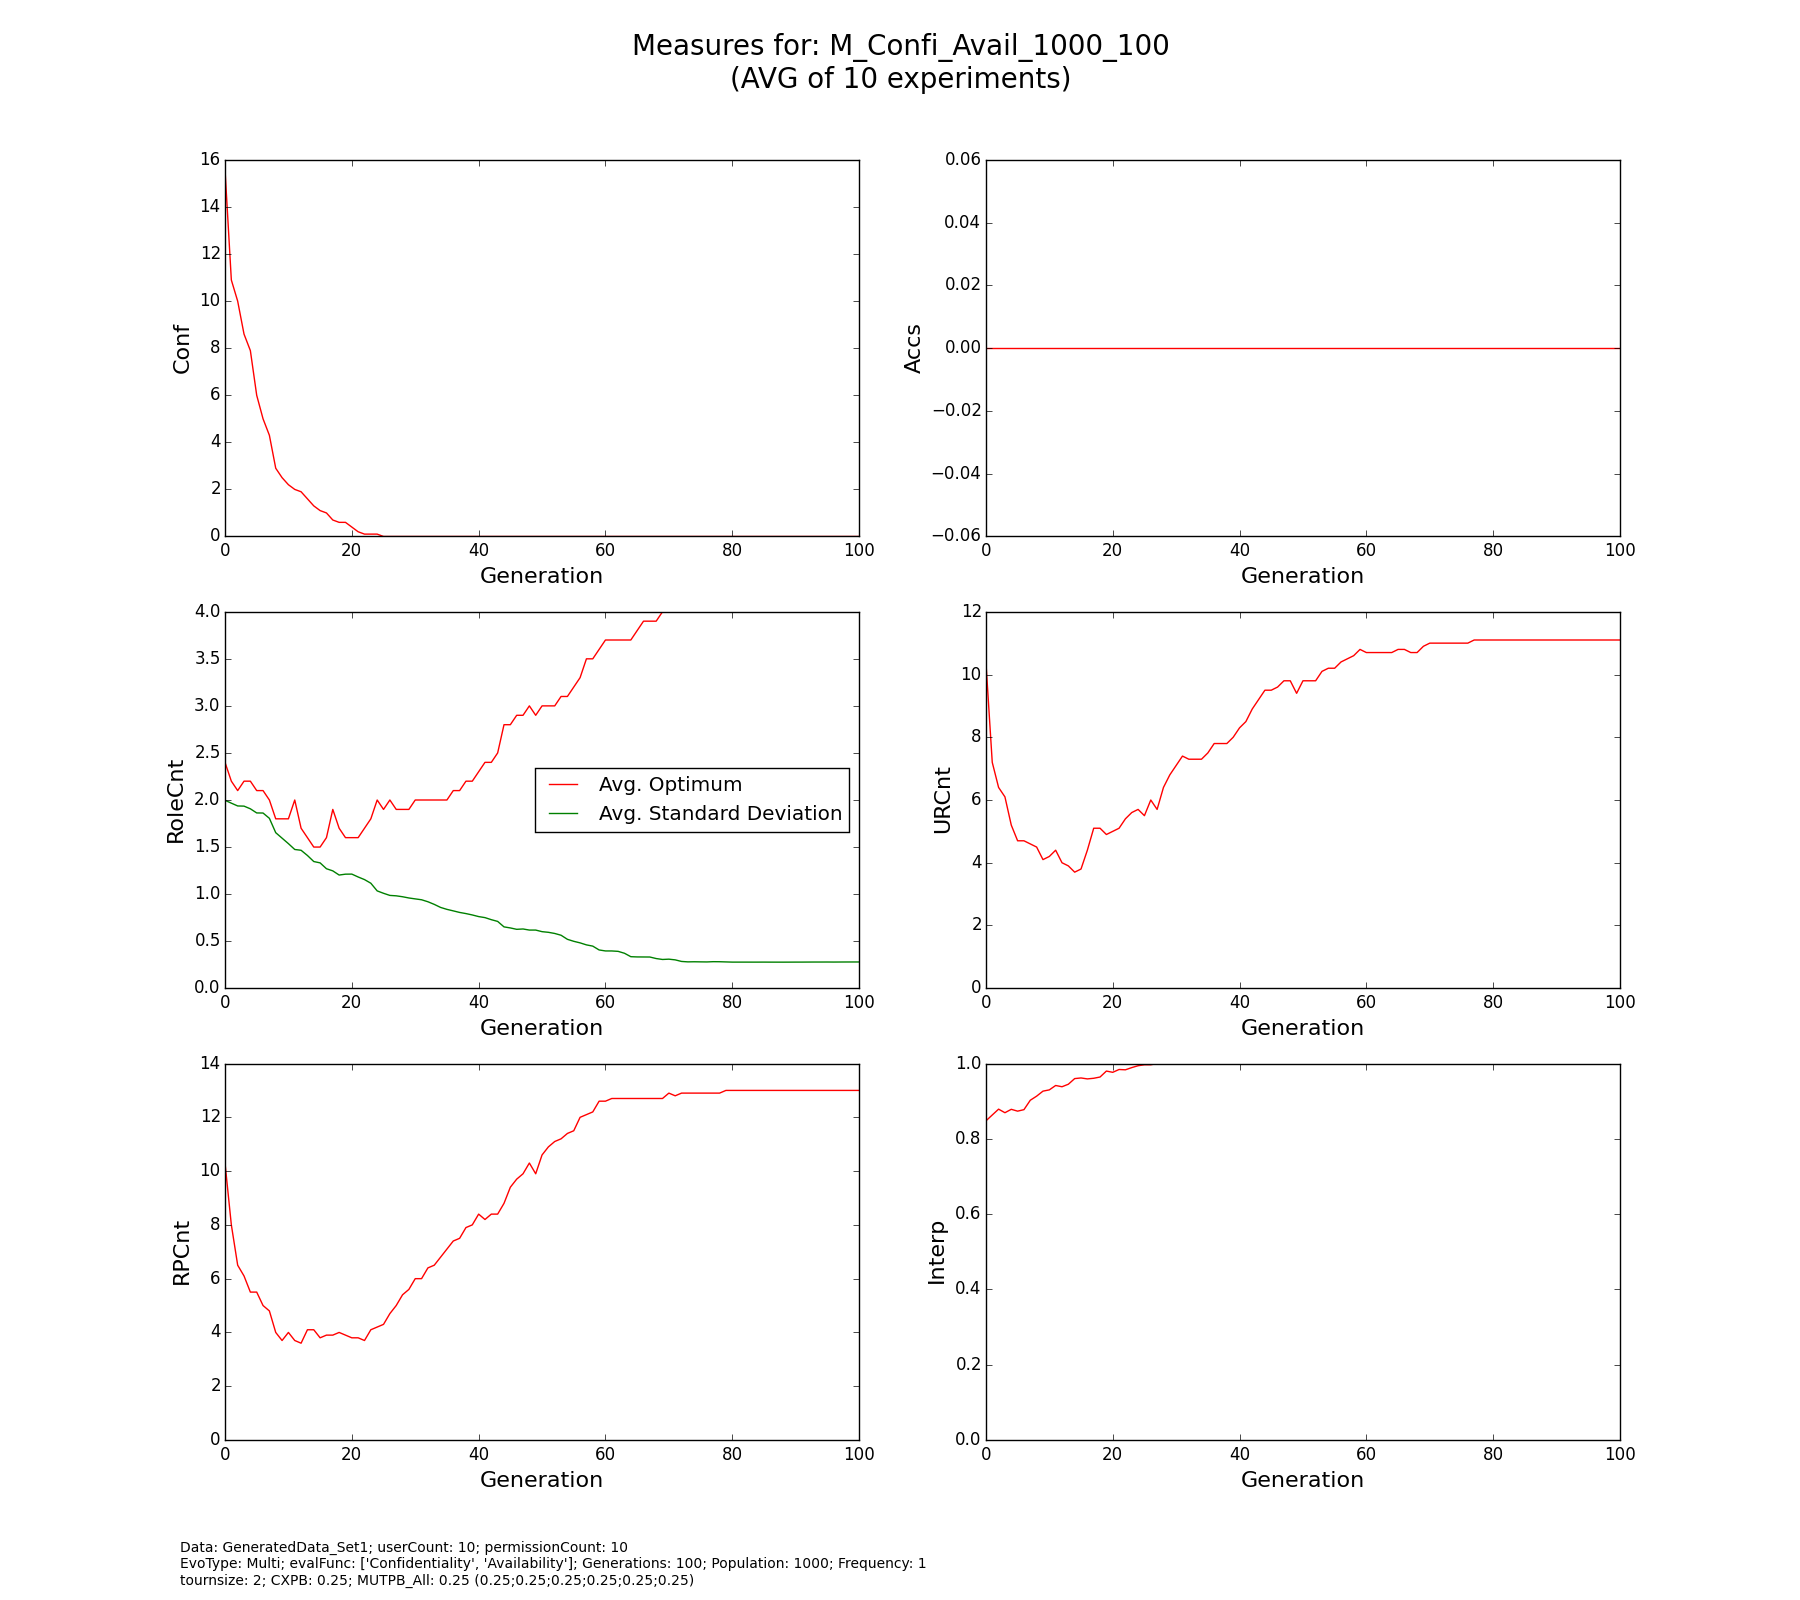
\includegraphics[scale=0.33, trim=4cm 2cm 4cm 0cm, clip=true]{exp4a_measures}
				\caption{EXPERIMENT 4a: Average optimum of the single objective measures of the ten experiments with Evo-RoleMiner$M$ on Dataset1}
				\label{fig:exp4a_measures}
			\end{figure}
			\begin{figure}[H]
				\centering
				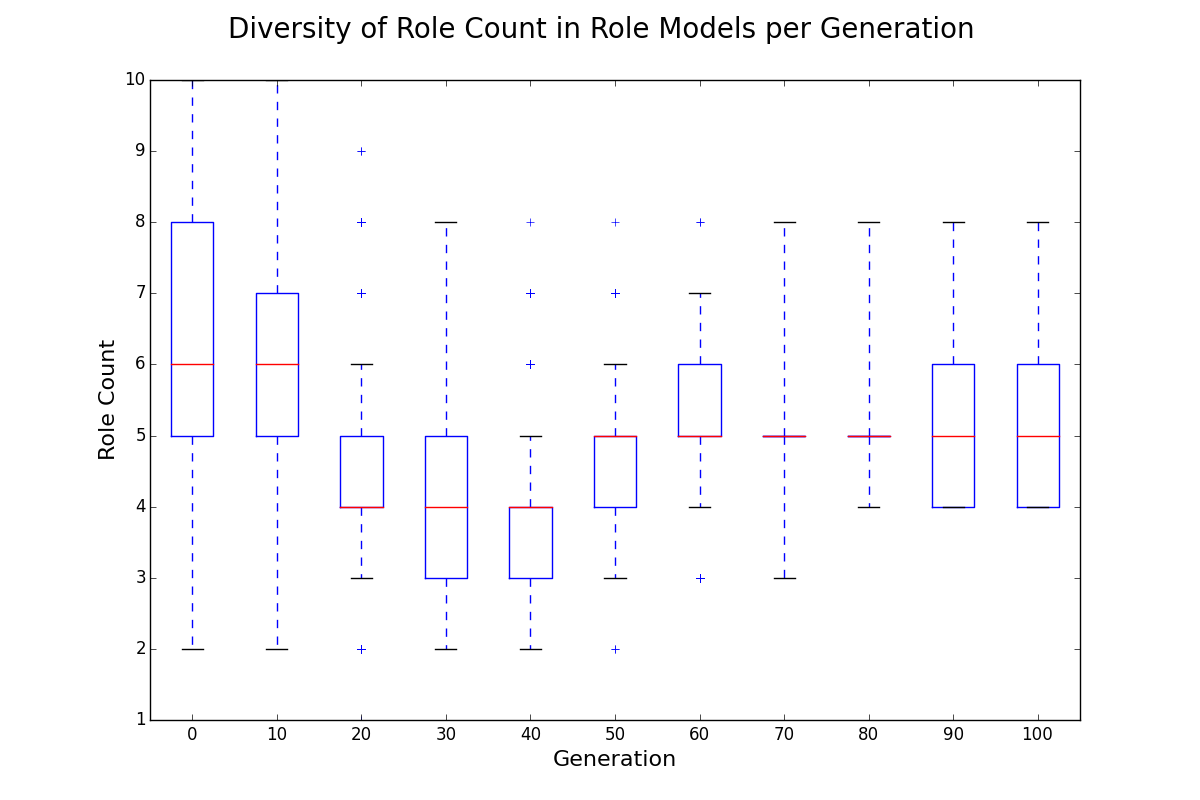
\includegraphics[scale=0.3]{exp4a_diversity}
				\caption{EXPERIMENT 4a: Example boxplot of role count diversity of individuals of a population in different generations with Evo-RoleMiner$M$ on Dataset1.}
				\label{fig:exp4a_diversity}
			\end{figure}

	\subsection{Experiment 4b}
	\label{sec:A_Exp4b}
		\subsubsection{Result Data}
		\label{sec:A_Exp4b_Data}
		\begin{table}[H]
			\caption{Results of Experiment 4b: Dataset1, NSGA-II$R$, Setup 4}
			\label{tab:A_Exp4b_Data}
			\begin{adjustbox}{max width=380pt,keepaspectratio,angle=90}
				\begin{tabular}{|l|l|l|l|l|l|l|l|l|l|l|}
					\hline
					\rowcolor[HTML]{EFEFEF} 
					Experiments & evals & Conf\_Min & Conf\_Max & Conf\_Avg & Conf\_Std & Accs\_Min & Accs\_Max & Accs\_Avg & Accs\_Std & RoleCnt\_Min \\ \hline
					\rowcolor[HTML]{FFFFFF} 
					1           & 1000  & 0         & 0         & 0         & 0         & 0         & 0         & 0         & 0         & 4            \\ \hline
					\rowcolor[HTML]{FFFFFF} 
					2           & 1000  & 0         & 0         & 0         & 0         & 0         & 0         & 0         & 0         & 4            \\ \hline
					\rowcolor[HTML]{FFFFFF} 
					3           & 1000  & 0         & 0         & 0         & 0         & 0         & 0         & 0         & 0         & 4            \\ \hline
					\rowcolor[HTML]{FFFFFF} 
					4           & 1000  & 0         & 0         & 0         & 0         & 0         & 0         & 0         & 0         & 4            \\ \hline
					\rowcolor[HTML]{FFFFFF} 
					5           & 1000  & 0         & 0         & 0         & 0         & 0         & 0         & 0         & 0         & 4            \\ \hline
					\rowcolor[HTML]{FFFFFF} 
					6           & 1000  & 0         & 0         & 0         & 0         & 0         & 0         & 0         & 0         & 4            \\ \hline
					\rowcolor[HTML]{FFFFFF} 
					7           & 1000  & 0         & 0         & 0         & 0         & 0         & 0         & 0         & 0         & 4            \\ \hline
					\rowcolor[HTML]{FFFFFF} 
					8           & 1000  & 0         & 0         & 0         & 0         & 0         & 0         & 0         & 0         & 4            \\ \hline
					\rowcolor[HTML]{FFFFFF} 
					9           & 1000  & 0         & 0         & 0         & 0         & 0         & 0         & 0         & 0         & 4            \\ \hline
					\rowcolor[HTML]{FFFFFF} 
					10          & 1000  & 0         & 0         & 0         & 0         & 0         & 0         & 0         & 0         & 4            \\ \hline
					\rowcolor[HTML]{FFFFFF} 
					AVG         & 1000  & 0         & 0         & 0         & 0         & 0         & 0         & 0         & 0         & 4            \\ \hline
				\end{tabular}
			\end{adjustbox}
			\begin{adjustbox}{max width=380pt,keepaspectratio,angle=90}
				\begin{tabular}{|l|l|l|l|l|l|l|l|l|l|l|}
					\hline
					\rowcolor[HTML]{EFEFEF} 
					Experiments & RoleCnt\_Max & RoleCnt\_Avg & RoleCnt\_Std & URCnt\_Min & URCnt\_Max & URCnt\_Avg & URCnt\_Std  & RPCnt\_Min & RPCnt\_Max & RPCnt\_Avg \\ \hline
					1           & 6            & 4.175        & 0.382589859  & 13         & 23         & 13.611     & 1.480432032 & 12         & 17         & 13.585     \\ \hline
					2           & 6            & 5.011        & 0.157730783  & 10         & 22         & 18.866     & 1.061152204 & 15         & 23         & 16.914     \\ \hline
					3           & 6            & 4.51         & 0.577840809  & 10         & 19         & 13.347     & 1.368426469 & 14         & 26         & 17.932     \\ \hline
					4           & 5            & 4.047        & 0.211638843  & 12         & 19         & 13.087     & 0.470564555 & 12         & 21         & 14.829     \\ \hline
					5           & 5            & 4.199        & 0.399248043  & 10         & 19         & 11.584     & 0.982315632 & 15         & 22         & 17.331     \\ \hline
					6           & 6            & 4.113        & 0.337980769  & 13         & 24         & 13.517     & 1.873955976 & 11         & 18         & 12.365     \\ \hline
					7           & 6            & 4.861        & 0.392019132  & 11         & 23         & 17.992     & 2.507974482 & 14         & 20         & 16.734     \\ \hline
					8           & 6            & 4.085        & 0.296268459  & 10         & 20         & 13.06      & 0.922171351 & 13         & 21         & 16.058     \\ \hline
					9           & 6            & 4.267        & 0.449122478  & 13         & 21         & 13.363     & 0.826577885 & 12         & 20         & 14.402     \\ \hline
					10          & 6            & 4.087        & 0.288844249  & 10         & 17         & 10.85      & 0.805915628 & 16         & 22         & 17.111     \\ \hline
					AVG         & 5.8          & 4.3355       & 0.349328342  & 11.2       & 20.7       & 13.9277    & 1.229948621 & 13.4       & 21         & 15.7261    \\ \hline
				\end{tabular}
			\end{adjustbox}
			\begin{adjustbox}{max width=340pt,keepaspectratio,angle=90}
				\begin{tabular}{|l|l|l|l|l|l|l|l|}
					\hline
					\rowcolor[HTML]{EFEFEF} 
					Experiments & RPCnt\_Std  & Interp\_Min & Interp\_Max & Interp\_Avg & Interp\_Std & Runtime     & Generation when Objectives are reached \\ \hline
					1           & 1.044401743 & 0.666666667 & 1           & 0.972746667 & 0.067174154 & 153.645712  & 23                                     \\ \hline
					2           & 0.6360849   & 0.78        & 1           & 0.957731667 & 0.01625463  & 395.101408  & 24                                     \\ \hline
					3           & 2.182974118 & 0.78        & 1           & 0.936465    & 0.078063051 & 412.185388  & 21                                     \\ \hline
					4           & 0.907611701 & 0.8         & 1           & 0.997465    & 0.017591156 & 531.735146  & 23                                     \\ \hline
					5           & 0.787044471 & 0.78        & 1           & 0.972       & 0.020654297 & 401.769795  & 23                                     \\ \hline
					6           & 0.719565841 & 0.8         & 1           & 0.98738     & 0.045313011 & 125.19408   & 21                                     \\ \hline
					7           & 0.628684341 & 0.78        & 1           & 0.943533333 & 0.054914115 & 144.290197  & 19                                     \\ \hline
					8           & 0.954272498 & 0.78        & 1           & 0.989538333 & 0.036481589 & 126.567993  & 27                                     \\ \hline
					9           & 1.316205151 & 0.8         & 1           & 0.988283333 & 0.022780541 & 138.144138  & 20                                     \\ \hline
					10          & 0.467631265 & 0.78        & 1           & 0.98082     & 0.017019591 & 135.587696  & 33                                     \\ \hline
					AVG         & 0.964447603 & 0.774666667 & 1           & 0.972596333 & 0.037624614 & 256.4221553 & 23.4                                   \\ \hline
				\end{tabular}
			\end{adjustbox}	
		\end{table}
	\subsection{Experiment 4c}
	\label{sec:A_Exp4c}
		\subsubsection{Result Data}
		\label{sec:A_Exp4c_Data}
		\begin{table}[H]
			\caption{Results of Experiment 4c: Dataset1, NSGA-II$R$ with weights, Setup 4}
			\label{tab:A_Exp4c_Data}
			\begin{adjustbox}{max width=480pt,keepaspectratio,angle=90}
				\begin{tabular}{|l|l|l|l|l|l|l|l|l|l|l|l|l|}
					\hline
					\rowcolor[HTML]{EFEFEF} 
					Experiments & evals & Violations\_Min & Violations\_Max & Violations\_Avg & Violations\_Std & AssignmentCnt\_Min & AssignmentCnt\_Max & AssignmentCnt\_Avg & AssignmentCnt\_Std & Conf\_Min & Conf\_Max & Conf\_Avg \\ \hline
					1           & 1000  & 0               & 0               & 0               & 0               & 25                 & 25                 & 25                 & 0                  & 0         & 0         & 0         \\ \hline
					2           & 1000  & 0               & 1               & 0.019           & 0.136524723     & 24                 & 26                 & 24.988             & 0.16079801         & 0         & 0         & 0         \\ \hline
					3           & 1000  & 0               & 1               & 0.02            & 0.14            & 24                 & 26                 & 24.994             & 0.184293245        & 0         & 0         & 0         \\ \hline
					4           & 1000  & 0               & 0               & 0               & 0               & 27                 & 27                 & 27                 & 0                  & 0         & 0         & 0         \\ \hline
					5           & 1000  & 0               & 0               & 0               & 0               & 25                 & 26                 & 25.105             & 0.306553421        & 0         & 0         & 0         \\ \hline
					6           & 1000  & 0               & 1               & 0.014           & 0.117490425     & 24                 & 26                 & 25.24              & 0.458693798        & 0         & 0         & 0         \\ \hline
					7           & 1000  & 0               & 0               & 0               & 0               & 25                 & 29                 & 25.004             & 0.126427845        & 0         & 0         & 0         \\ \hline
					8           & 1000  & 0               & 1               & 0.041           & 0.198290191     & 24                 & 28                 & 24.971             & 0.245273317        & 0         & 0         & 0         \\ \hline
					9           & 1000  & 0               & 0               & 0               & 0               & 25                 & 27                 & 25.129             & 0.361052628        & 0         & 0         & 0         \\ \hline
					10          & 1000  & 0               & 1               & 0.058           & 0.233743449     & 24                 & 25                 & 24.942             & 0.233743449        & 0         & 0         & 0         \\ \hline
					AVG         & 1000  & 0               & 0.5             & 0.0152          & 0.082604879     & 24.7               & 26.5               & 25.2373            & 0.207683571        & 0         & 0         & 0         \\ \hline
				\end{tabular}
			\end{adjustbox}
			\begin{adjustbox}{max width=480pt,keepaspectratio,angle=90}
				\begin{tabular}{|l|l|l|l|l|l|l|l|l|l|l|l|l|}
					\hline
					\rowcolor[HTML]{EFEFEF} 
					Experiments & Conf\_Std & Accs\_Min & Accs\_Max & Accs\_Avg & Accs\_Std   & RoleCnt\_Min & RoleCnt\_Max & RoleCnt\_Avg & RoleCnt\_Std & URCnt\_Min & URCnt\_Max & URCnt\_Avg \\ \hline
					1           & 0         & 0         & 0         & 0         & 0           & 4            & 4            & 4            & 0            & 13         & 13         & 13         \\ \hline
					2           & 0         & 0         & 1         & 0.019     & 0.136524723 & 4            & 4            & 4            & 0            & 13         & 13         & 13         \\ \hline
					3           & 0         & 0         & 1         & 0.02      & 0.14        & 4            & 4            & 4            & 0            & 13         & 13         & 13         \\ \hline
					4           & 0         & 0         & 0         & 0         & 0           & 4            & 4            & 4            & 0            & 10         & 10         & 10         \\ \hline
					5           & 0         & 0         & 0         & 0         & 0           & 4            & 4            & 4            & 0            & 13         & 13         & 13         \\ \hline
					6           & 0         & 0         & 1         & 0.014     & 0.117490425 & 4            & 4            & 4            & 0            & 13         & 13         & 13         \\ \hline
					7           & 0         & 0         & 0         & 0         & 0           & 4            & 5            & 4.001        & 0.031606961  & 13         & 15         & 13.002     \\ \hline
					8           & 0         & 0         & 1         & 0.041     & 0.198290191 & 4            & 5            & 4.002        & 0.044676616  & 13         & 14         & 13.002     \\ \hline
					9           & 0         & 0         & 0         & 0         & 0           & 4            & 4            & 4            & 0            & 13         & 13         & 13         \\ \hline
					10          & 0         & 0         & 1         & 0.058     & 0.233743449 & 4            & 4            & 4            & 0            & 13         & 13         & 13         \\ \hline
					AVG         & 0         & 0         & 0.5       & 0.0152    & 0.082604879 & 4            & 4.2          & 4.0003       & 0.007628358  & 12.7       & 13         & 12.7004    \\ \hline
				\end{tabular}
			\end{adjustbox}
			\begin{adjustbox}{max width=460pt,keepaspectratio,angle=90}
				\begin{tabular}{|l|l|l|l|l|l|l|l|l|l|l|l|}
					\hline
					\rowcolor[HTML]{EFEFEF} 
					Experiments & URCnt\_Std  & RPCnt\_Min & RPCnt\_Max & RPCnt\_Avg & RPCnt\_Std  & Interp\_Min & Interp\_Max & Interp\_Avg & Interp\_Std & Runtime     & Generation when Objectives are reached \\ \hline
					1           & 0           & 12         & 12         & 12         & 0           & 1           & 1           & 1           & 0           & 147.777375  & 23                                     \\ \hline
					2           & 0           & 11         & 13         & 11.988     & 0.16079801  & 1           & 1           & 1           & 0           & 150.971537  & 24                                     \\ \hline
					3           & 0           & 11         & 13         & 11.994     & 0.184293245 & 1           & 1           & 1           & 0           & 134.201258  & 29                                     \\ \hline
					4           & 0           & 17         & 17         & 17         & 0           & 1           & 1           & 1           & 0           & 128.918312  & 21                                     \\ \hline
					5           & 0           & 12         & 13         & 12.105     & 0.306553421 & 1           & 1           & 1           & 0           & 133.957595  & 28                                     \\ \hline
					6           & 0           & 11         & 13         & 12.24      & 0.458693798 & 1           & 1           & 1           & 0           & 126.298156  & 22                                     \\ \hline
					7           & 0.063213923 & 12         & 14         & 12.002     & 0.063213923 & 1           & 1           & 1           & 0           & 159.747057  & 32                                     \\ \hline
					8           & 0.044676616 & 11         & 14         & 11.969     & 0.228120582 & 0.96        & 1           & 0.99994     & 0.00141294  & 136.910545  & 30                                     \\ \hline
					9           & 0           & 12         & 14         & 12.129     & 0.361052628 & 1           & 1           & 1           & 0           & 133.527571  & 25                                     \\ \hline
					10          & 0           & 11         & 12         & 11.942     & 0.233743449 & 1           & 1           & 1           & 0           & 134.280632  & 28                                     \\ \hline
					AVG         & 0.010789054 & 12         & 13.5       & 12.5369    & 0.199646905 & 0.996       & 1           & 0.999994    & 0.000141294 & 138.6590038 & 26.2                                   \\ \hline
				\end{tabular}
			\end{adjustbox}	
		\end{table}	
	\subsection{Experiment 4d}
	\label{sec:A_Exp4d}
		\subsubsection{Result Data}
		\label{sec:A_Exp4d_Data}
		\begin{table}[H]
			\caption{Results of Experiment 4d: Healthcare, NSGA-II, Setup 4}
			\label{tab:A_Exp4d_Data}
			\begin{adjustbox}{max width=360pt,keepaspectratio,angle=90}
				\begin{tabular}{|l|l|l|l|l|l|l|l|l|l|}
					\hline
					\rowcolor[HTML]{EFEFEF} 
					Experiments & Conf\_Min & Conf\_Max & Conf\_Avg & Conf\_Std   & Accs\_Min & Accs\_Max & Accs\_Avg & Accs\_Std   & RoleCnt\_Min \\ \hline
					1           & 0         & 2         & 1         & 1           & 0         & 1         & 0.5       & 0.5         & 20           \\ \hline
					2           & 0         & 5         & 2.287     & 2.034362554 & 0         & 3         & 1.357     & 1.2318892   & 17           \\ \hline
					3           & 0         & 5         & 2.526     & 2.430498714 & 0         & 2         & 1.001     & 0.971081356 & 19           \\ \hline
					4           & 0         & 0         & 0         & 0           & 0         & 0         & 0         & 0           & 18           \\ \hline
					5           & 0         & 0         & 0         & 0           & 0         & 0         & 0         & 0           & 20           \\ \hline
					6           & 0         & 0         & 0         & 0           & 0         & 0         & 0         & 0           & 18           \\ \hline
					7           & 0         & 0         & 0         & 0           & 0         & 0         & 0         & 0           & 20           \\ \hline
					8           & 0         & 1         & 0.5       & 0.5         & 0         & 2         & 1         & 1           & 15           \\ \hline
					9           & 0         & 2         & 1         & 1           & 0         & 1         & 0.5       & 0.5         & 21           \\ \hline
					10          & 0         & 0         & 0         & 0           & 0         & 0         & 0         & 0           & 20           \\ \hline
					AVG         & 0         & 1.5       & 0.7313    & 0.696486127 & 0         & 0.9       & 0.4358    & 0.420297056 & 18.8         \\ \hline
				\end{tabular}
			\end{adjustbox}
			\begin{adjustbox}{max width=360pt,keepaspectratio,angle=90}
				\begin{tabular}{|l|l|l|l|l|l|l|l|l|l|}
					\hline
					\rowcolor[HTML]{EFEFEF} 
					Experiments & RoleCnt\_Max & RoleCnt\_Avg & RoleCnt\_Std & URCnt\_Min & URCnt\_Max & URCnt\_Avg & URCnt\_Std  & RPCnt\_Min & RPCnt\_Max \\ \hline
					1           & 23           & 21.894       & 0.398452005  & 266        & 303        & 273.216    & 3.149181481 & 303        & 351        \\ \hline
					2           & 19           & 17.117       & 0.362368597  & 224        & 270        & 231.296    & 5.542236372 & 221        & 254        \\ \hline
					3           & 23           & 19.183       & 0.521067174  & 290        & 344        & 297.031    & 3.800005132 & 265        & 299        \\ \hline
					4           & 20           & 18.934       & 0.282212686  & 213        & 246        & 219.712    & 1.916       & 228        & 282        \\ \hline
					5           & 21           & 20.018       & 0.132951119  & 235        & 267        & 238.038    & 1.997136951 & 299        & 309        \\ \hline
					6           & 19           & 18.011       & 0.104302445  & 203        & 230        & 209.828    & 1.564102298 & 258        & 276        \\ \hline
					7           & 22           & 20.969       & 0.253059282  & 229        & 271        & 239.592    & 2.420234699 & 354        & 366        \\ \hline
					8           & 18           & 16.183       & 0.597922236  & 160        & 210        & 184.449    & 11.66350715 & 237        & 268        \\ \hline
					9           & 22           & 21.045       & 0.207304124  & 278        & 309        & 283.795    & 2.965295095 & 272        & 308        \\ \hline
					10          & 22           & 21.013       & 0.137226091  & 277        & 320        & 293.078    & 2.063471832 & 230        & 265        \\ \hline
					AVG         & 20.9         & 19.4367      & 0.299686576  & 237.5      & 277        & 247.0035   & 3.708117101 & 266.7      & 297.8      \\ \hline
				\end{tabular}
			\end{adjustbox}
			\begin{adjustbox}{max width=300pt,keepaspectratio,angle=90}
				\begin{tabular}{|l|l|l|l|l|l|l|l|l|}
					\hline
					\rowcolor[HTML]{EFEFEF} 
					Experiments & RPCnt\_Avg & RPCnt\_Std  & Interp\_Min & Interp\_Max & Interp\_Avg & Interp\_Std & Runtime     & Gamma \\ \hline
					1           & 323.73     & 4.981475685 & 0           & 0           & 0           & 0           & 3830.31913  & None  \\ \hline
					2           & 227.359    & 3.415570084 & 0           & 0           & 0           & 0           & 3443.911226 & None  \\ \hline
					3           & 276.515    & 5.038826748 & 0           & 0           & 0           & 0           & 3955.861228 & None  \\ \hline
					4           & 251.3      & 6.192091731 & 0           & 0           & 0           & 0           & 3605.379102 & 696   \\ \hline
					5           & 302.986    & 1.164389969 & 0           & 0           & 0           & 0           & 3999.715123 & 578   \\ \hline
					6           & 262.8      & 1.299230542 & 0           & 0           & 0           & 0           & 3578.616864 & 774   \\ \hline
					7           & 360.512    & 1.621066316 & 0           & 0           & 0           & 0           & 4182.867743 & 793   \\ \hline
					8           & 241.838    & 2.318567661 & 0           & 0           & 0           & 0           & 3246.070478 & None  \\ \hline
					9           & 278.75     & 4.371212646 & 0           & 0           & 0           & 0           & 3901.098761 & None  \\ \hline
					10          & 236.304    & 2.127342004 & 0           & 0           & 0           & 0           & 3914.201339 & 948   \\ \hline
					AVG         & 276.2094   & 3.252977339 & 0           & 0           & 0           & 0           & 3765.804099 & 757.8 \\ \hline
				\end{tabular}
			\end{adjustbox}	
		\end{table}
		\subsubsection{Result Visualizations}
		\label{sec:A_Exp4d_Diagrams}
			\begin{figure}[H]
				\centering
				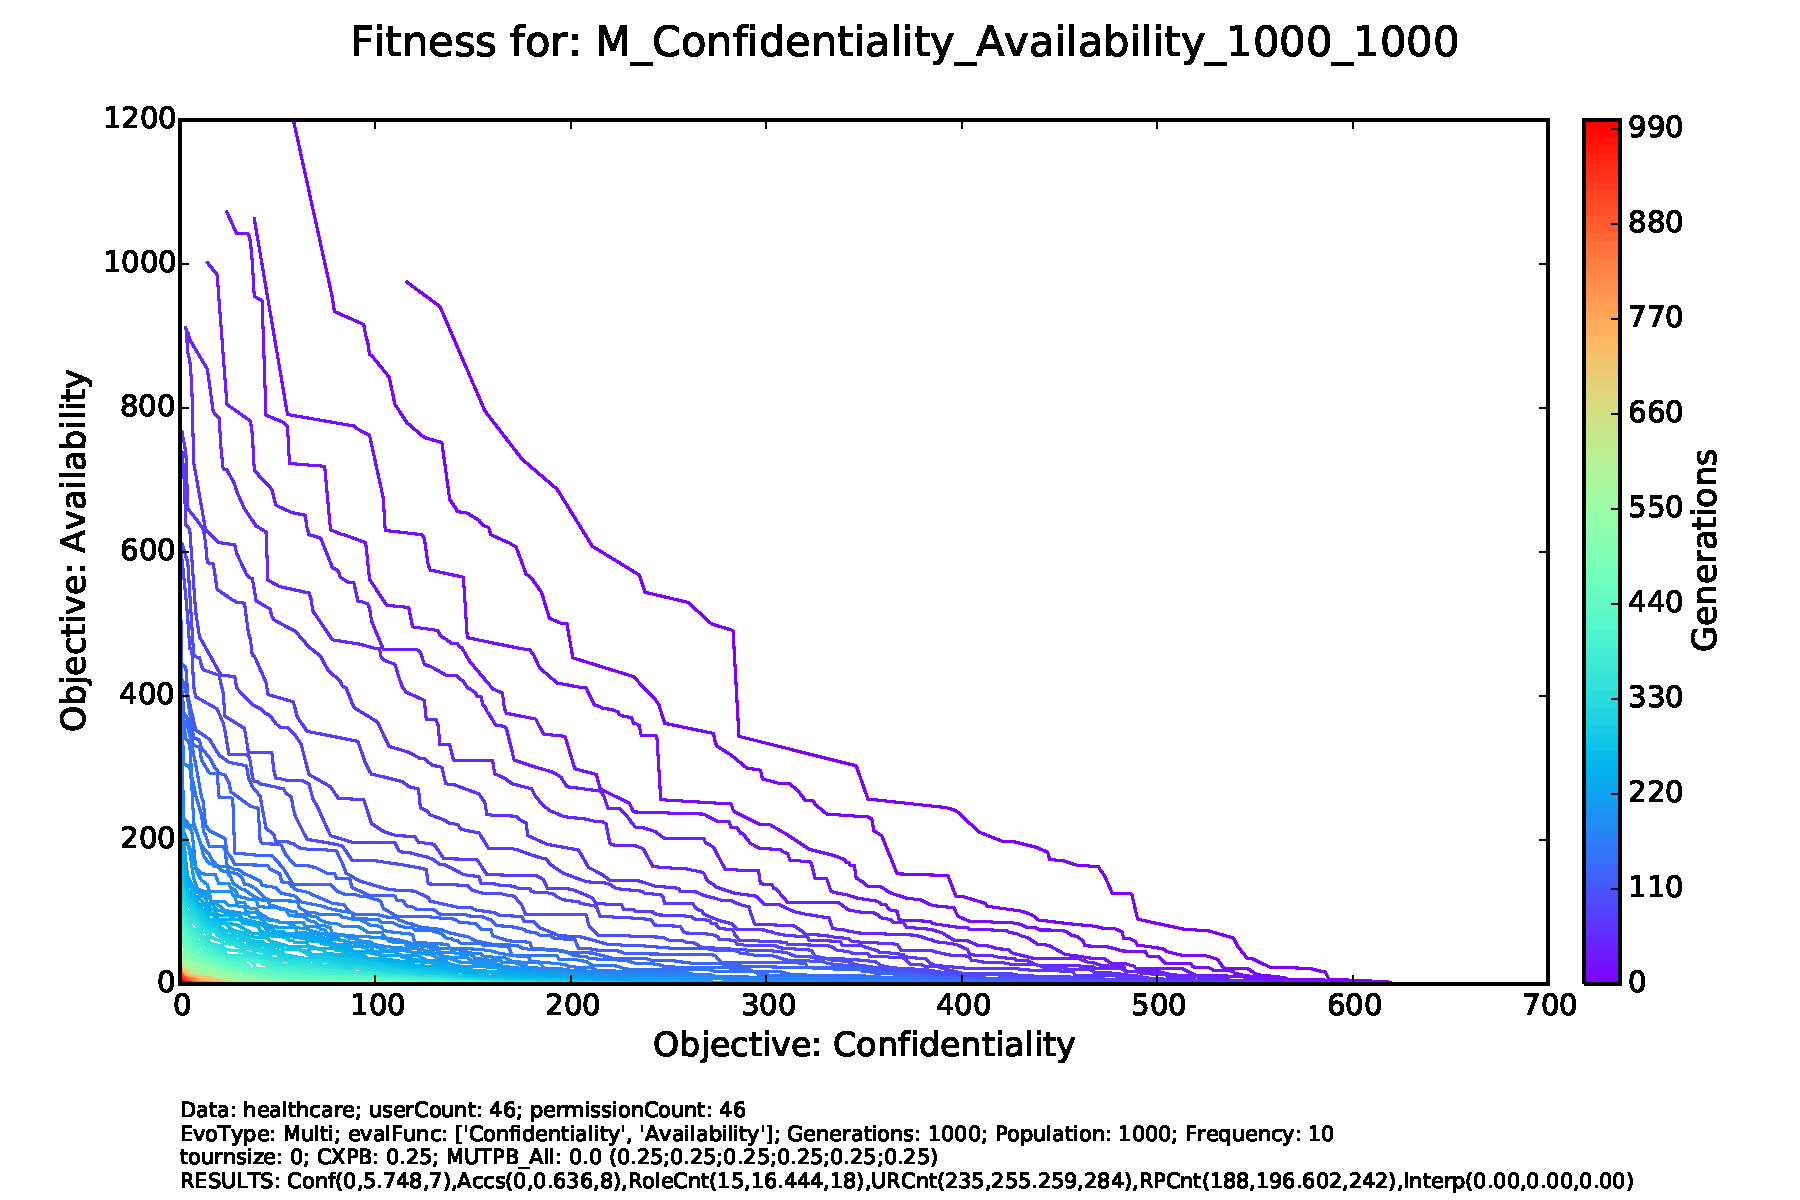
\includegraphics[width=\textwidth, trim=0cm 2cm 0cm 1.5cm, clip=true]{exp4d_fitness_pareto}
				\caption{EXPERIMENT 4d: Example of result of the experiments with Evo-RoleMiner$M$ (based on NSGA-II) on the Healthcare dataset. Illustrates the pareto fronts of each generation.}
				\label{fig:exp4d_fitness_pareto}
			\end{figure}
			\begin{figure}[H]
				\centering
				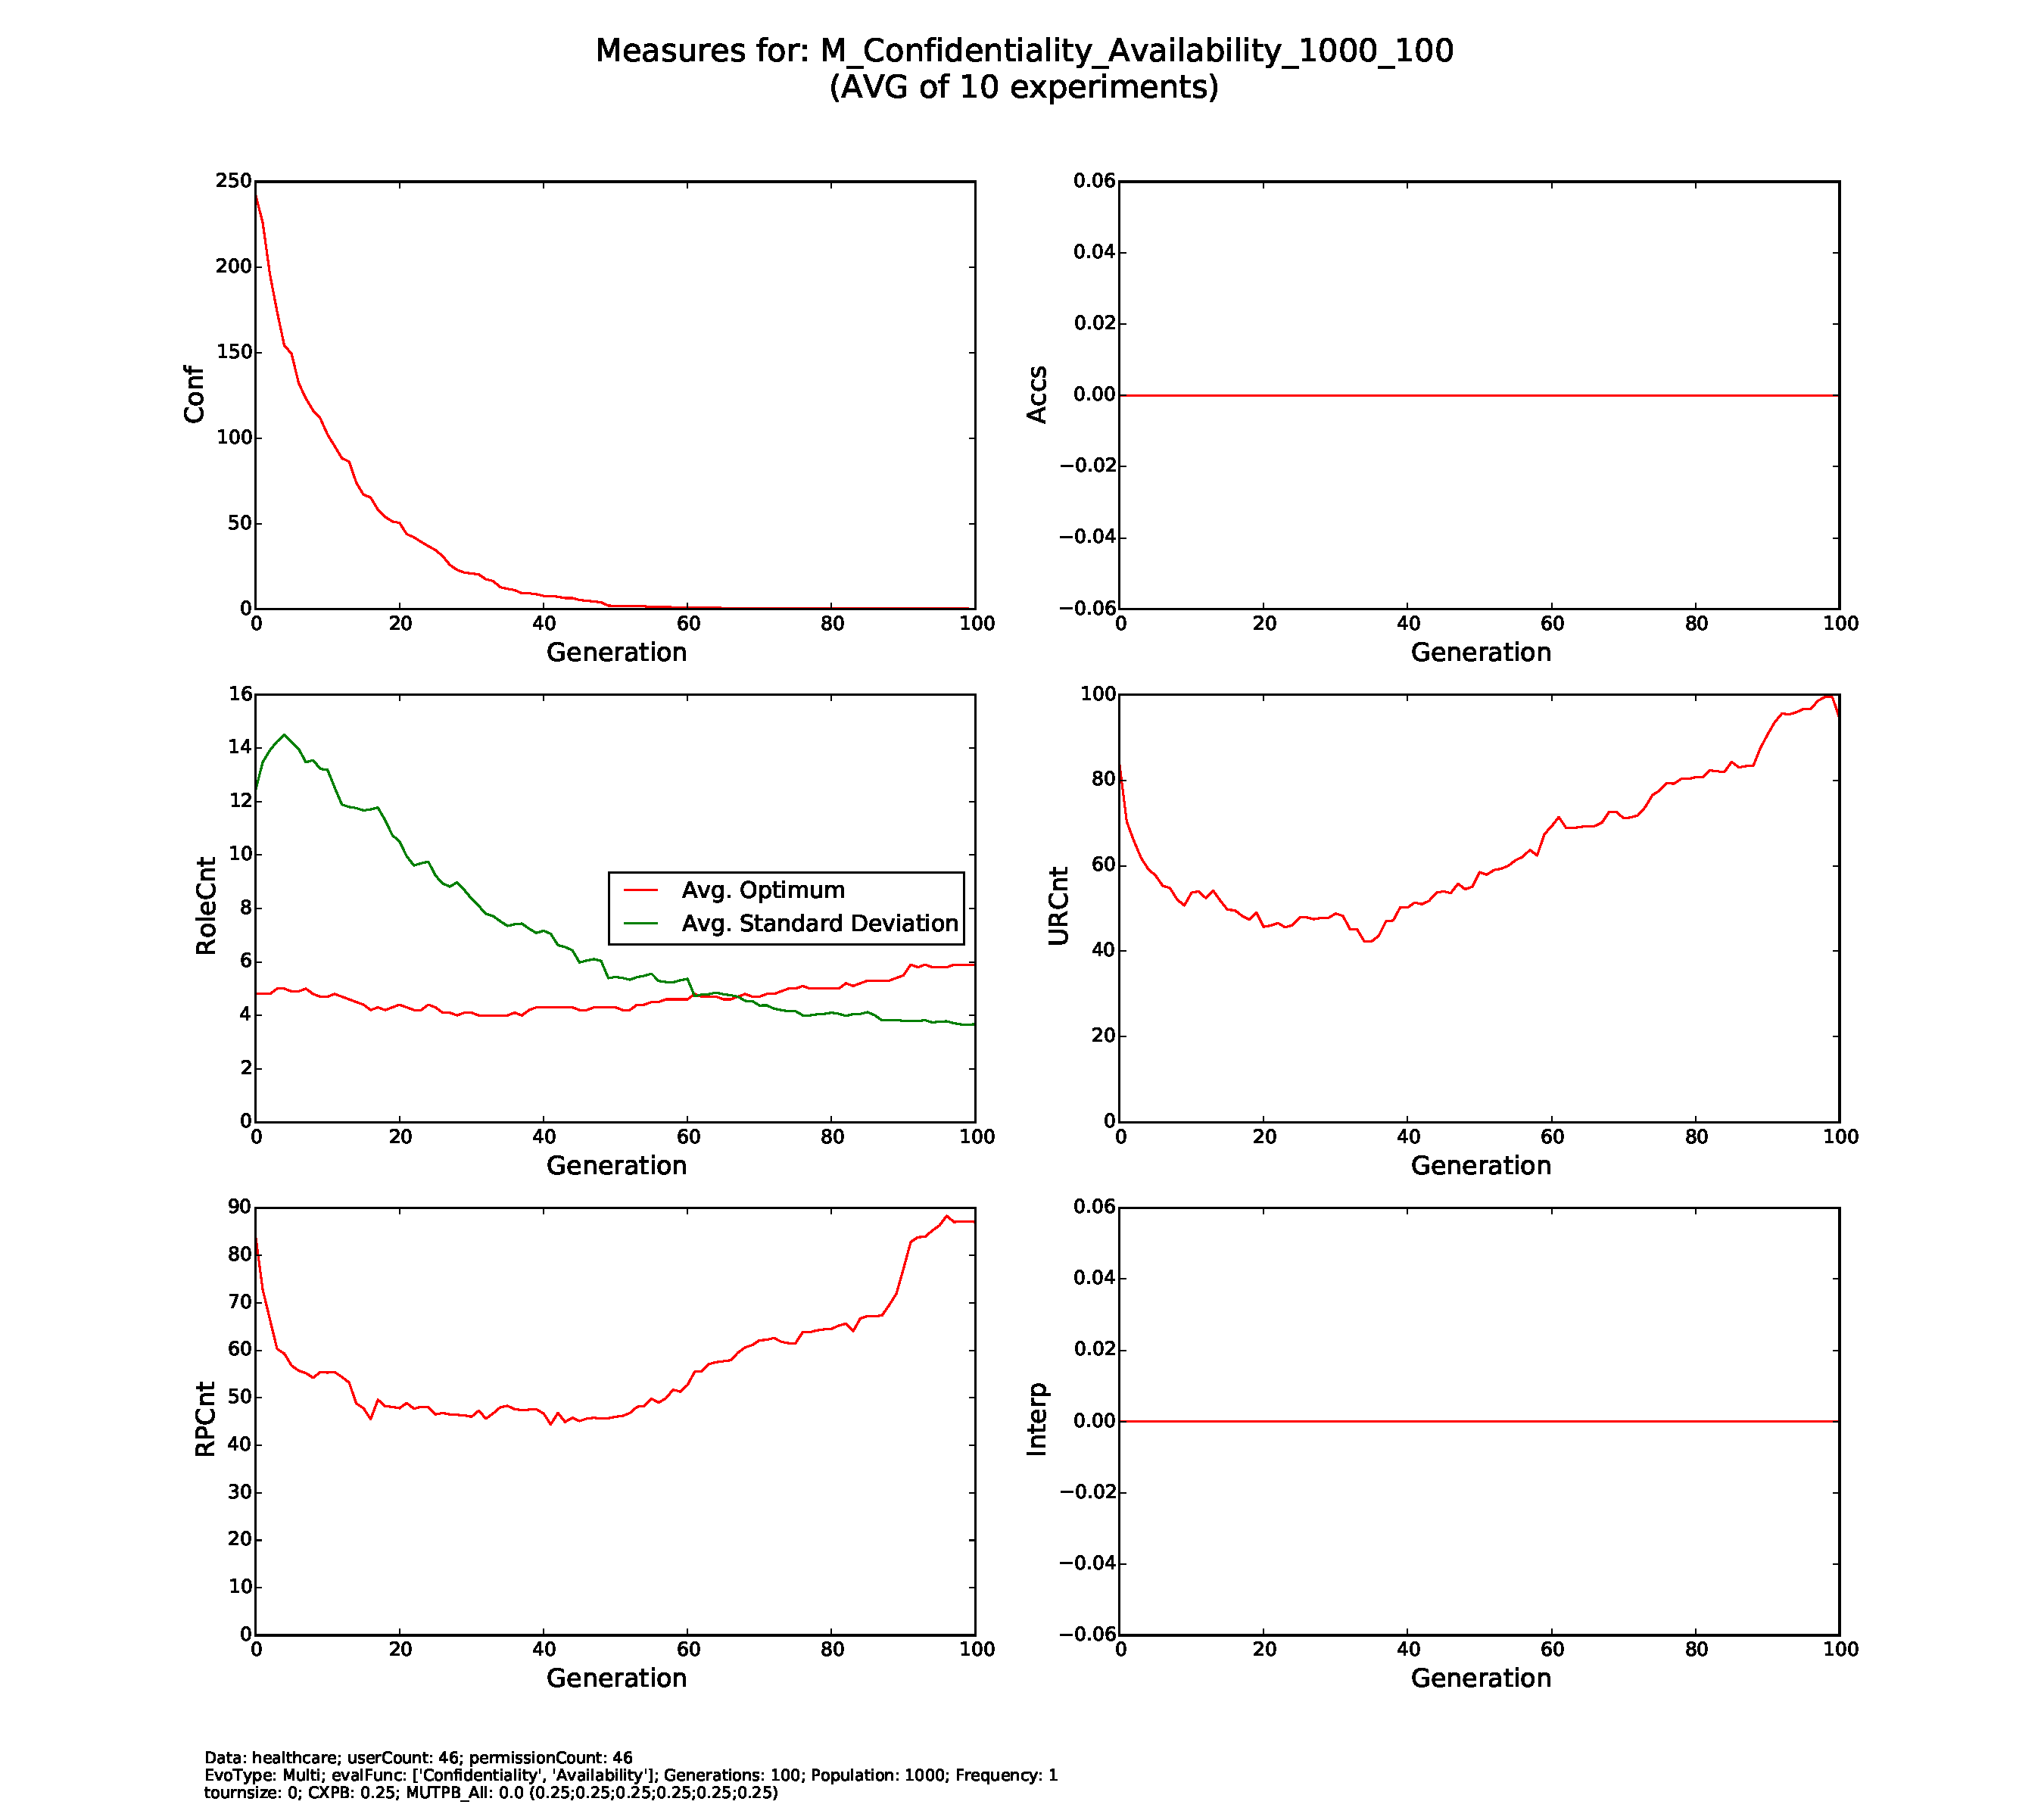
\includegraphics[scale=0.33, trim=4cm 2cm 4cm 0cm, clip=true]{exp4d_measures}
				\caption{EXPERIMENT 4d: Average optimum of the single objective measures of the ten experiments with Evo-RoleMiner$M$ on the healthcare dataset. The Interpretability measure is not activated and therefore constantly zero.}
				\label{fig:exp4d_measures}
			\end{figure}
			
	\subsection{Experiment 4e}
	\label{sec:A_Exp4e}
	\subsubsection{Result Data}
	\label{sec:A_Exp4e_Data}
	\begin{table}[H]
		\caption{Results of Experiment 4e: Healthcare, NSGA-II$R$, Setup 3}
		\label{tab:A_Exp4e_Data}
		\begin{adjustbox}{max width=380pt,keepaspectratio,angle=90}
			\begin{tabular}{|l|l|l|l|l|l|l|l|l|l|l|}
				\hline
				\rowcolor[HTML]{EFEFEF} 
				Experiments & evals & Conf\_Min & Conf\_Max & Conf\_Avg & Conf\_Std   & Accs\_Min & Accs\_Max & Accs\_Avg & Accs\_Std   & RoleCnt\_Min \\ \hline
				1           & 1000  & 0         & 0         & 0         & 0           & 0         & 0         & 0         & 0           & 18           \\ \hline
				2           & 1000  & 0         & 0         & 0         & 0           & 0         & 0         & 0         & 0           & 19           \\ \hline
				3           & 1000  & 0         & 3         & 1.5       & 1.118033989 & 0         & 4         & 1.75      & 1.479019946 & 17           \\ \hline
				4           & 1000  & 0         & 0         & 0         & 0           & 0         & 0         & 0         & 0           & 18           \\ \hline
				5           & 1000  & 0         & 0         & 0         & 0           & 0         & 0         & 0         & 0           & 18           \\ \hline
				6           & 1000  & 0         & 0         & 0         & 0           & 0         & 0         & 0         & 0           & 18           \\ \hline
				7           & 1000  & 0         & 0         & 0         & 0           & 0         & 0         & 0         & 0           & 19           \\ \hline
				8           & 1000  & 0         & 1         & 0.5       & 0.5         & 0         & 1         & 0.5       & 0.5         & 19           \\ \hline
				9           & 1000  & 0         & 0         & 0         & 0           & 0         & 0         & 0         & 0           & 19           \\ \hline
				10          & 1000  & 0         & 1         & 0.5       & 0.5         & 0         & 1         & 0.5       & 0.5         & 21           \\ \hline
				AVG         & 1000  & 0         & 0.5       & 0.25      & 0.211803399 & 0         & 0.6       & 0.275     & 0.247901995 & 18.6         \\ \hline
			\end{tabular}
		\end{adjustbox}
		\begin{adjustbox}{max width=380pt,keepaspectratio,angle=90}
			\begin{tabular}{|l|l|l|l|l|l|l|l|l|l|l|}
				\hline
				\rowcolor[HTML]{EFEFEF} 
				Experiments & RoleCnt\_Max & RoleCnt\_Avg & RoleCnt\_Std & URCnt\_Min & URCnt\_Max & URCnt\_Avg & URCnt\_Std  & RPCnt\_Min & RPCnt\_Max & RPCnt\_Avg \\ \hline
				1           & 19           & 18.035       & 0.183779759  & 227        & 258        & 232.01     & 2.527033834 & 275        & 308        & 279.182    \\ \hline
				2           & 21           & 19.048       & 0.227367544  & 284        & 321        & 289.44     & 4.41320745  & 236        & 264        & 240.031    \\ \hline
				3           & 22           & 17.582       & 0.865607301  & 258        & 315        & 274.498    & 8.424725277 & 224        & 287        & 238.928    \\ \hline
				4           & 22           & 20.682       & 0.613902272  & 234        & 271        & 240.715    & 3.365676009 & 283        & 365        & 338.951    \\ \hline
				5           & 20           & 19.02        & 0.278567766  & 189        & 215        & 194.045    & 2.100708214 & 281        & 320        & 287.712    \\ \hline
				6           & 21           & 18.92        & 0.381575681  & 229        & 266        & 233.833    & 2.605208437 & 265        & 301        & 271.98     \\ \hline
				7           & 21           & 19.921       & 0.383091373  & 254        & 290        & 260.874    & 3.267739892 & 266        & 307        & 275.21     \\ \hline
				8           & 21           & 19.871       & 0.533253223  & 208        & 252        & 230.128    & 9.683677814 & 311        & 369        & 343.169    \\ \hline
				9           & 20           & 19.024       & 0.153049012  & 252        & 282        & 256.847    & 2.178437743 & 298        & 327        & 302.1      \\ \hline
				10          & 23           & 22.07        & 0.401372645  & 287        & 323        & 294.353    & 5.205995678 & 301        & 339        & 313.923    \\ \hline
				AVG         & 21           & 19.4173      & 0.402156658  & 242.2      & 279.3      & 250.6743   & 4.377241035 & 274        & 318.7      & 289.1186   \\ \hline
			\end{tabular}
		\end{adjustbox}
		\begin{adjustbox}{max width=340pt,keepaspectratio,angle=90}
			\begin{tabular}{|l|l|l|l|l|l|l|l|l|l|l|}
				\hline
				\rowcolor[HTML]{EFEFEF} 
				Experiments & RPCnt\_Std  & Interp\_Min & Interp\_Max & Interp\_Avg & Interp\_Std & Runtime     & solutionFound & solutionFound &   &          \\ \hline
				1           & 2.459446279 & 0           & 0           & 0           & 0           & 7004.041559 & 729           & "{[}111       & 1 & 729{]}"  \\ \hline
				2           & 2.134019447 & 0           & 0           & 0           & 0           & 7270.995842 & 804           & "{[}77        & 1 & 804{]}"  \\ \hline
				3           & 8.305709843 & 0           & 0           & 0           & 0           & 7167.064926 &               & "{[}34        & 1 & None{]}" \\ \hline
				4           & 13.63020906 & 0           & 0           & 0           & 0           & 7805.748457 & 898           & "{[}55        & 1 & 898{]}"  \\ \hline
				5           & 3.779822218 & 0           & 0           & 0           & 0           & 6869.585912 & 1522          & "{[}70        & 1 & 1522{]}" \\ \hline
				6           & 2.89786128  & 0           & 0           & 0           & 0           & 7261.956335 & 696           & "{[}113       & 1 & 696{]}"  \\ \hline
				7           & 3.948658    & 0           & 0           & 0           & 0           & 7310.509125 & 1114          & "{[}54        & 1 & 1114{]}" \\ \hline
				8           & 4.443696547 & 0           & 0           & 0           & 0           & 7674.168937 &               & "{[}69        & 1 & None{]}" \\ \hline
				9           & 1.962651268 & 0           & 0           & 0           & 0           & 7585.876887 & 610           & "{[}48        & 1 & 610{]}"  \\ \hline
				10          & 4.916815128 & 0           & 0           & 0           & 0           & 8128.169905 &               & "{[}92        & 1 & None{]}" \\ \hline
				AVG         & 4.847888907 & 0           & 0           & 0           & 0           & 7407.811789 & 910.4285714   &               &   &          \\ \hline
			\end{tabular}
		\end{adjustbox}	
	\end{table}
			
	\subsection{Experiment 4f}
	\label{sec:A_Exp4f}
	\subsubsection{Result Data}
	\label{sec:A_Exp4f_Data}	
			\begin{table}[H]
				\caption{Results of Experiment 4f: Healthcare, NSGA-II$R$ with weights, Setup 3}
				\label{tab:A_Exp4f_Data}
				\begin{adjustbox}{max width=480pt,keepaspectratio,angle=90}
				\begin{tabular}{|l|l|l|l|l|l|l|l|l|l|l|l|l|l|}
					\hline
					\rowcolor[HTML]{EFEFEF} 
					Experiments & evals & Violations\_Min & Violations\_Max & Violations\_Avg & Violations\_Std & AssignmentCnt\_Min & AssignmentCnt\_Max & AssignmentCnt\_Avg & AssignmentCnt\_Std & Conf\_Min & Conf\_Max & Conf\_Avg & Conf\_Std   \\ \hline
					1           & 1000  & 17              & 18              & 17.01           & 0.099498744     & 322                & 324                & 323.026            & 0.21289434         & 15        & 15        & 15        & 0           \\ \hline
					2           & 1000  & 31              & 31              & 31              & 0               & 279                & 279                & 279                & 0                  & 14        & 14        & 14        & 0           \\ \hline
					3           & 1000  & 10              & 12              & 10.004          & 0.089353232     & 336                & 339                & 338.994            & 0.134029847        & 8         & 8         & 8         & 0           \\ \hline
					4           & 1000  & 5               & 5               & 5               & 0               & 254                & 255                & 254.015            & 0.121552458        & 1         & 1         & 1         & 0           \\ \hline
					5           & 1000  & 20              & 20              & 20              & 0               & 277                & 277                & 277                & 0                  & 17        & 17        & 17        & 0           \\ \hline
					6           & 1000  & 11              & 11              & 11              & 0               & 310                & 310                & 310                & 0                  & 3         & 3         & 3         & 0           \\ \hline
					7           & 1000  & 15              & 16              & 15.305          & 0.460407428     & 288                & 289                & 288.695            & 0.460407428        & 10        & 10        & 10        & 0           \\ \hline
					8           & 1000  & 3               & 4               & 3.023           & 0.149903302     & 304                & 307                & 304.987            & 0.206956517        & 3         & 3         & 3         & 0           \\ \hline
					9           & 1000  & 15              & 15              & 15              & 0               & 366                & 366                & 366                & 0                  & 12        & 12        & 12        & 0           \\ \hline
					10          & 1000  & 14              & 14              & 14              & 0               & 263                & 264                & 263.377            & 0.484634914        & 0         & 2         & 0.002     & 0.063213923 \\ \hline
					AVG         & 1000  & 14.1            & 14.6            & 14.1342         & 0.079916271     & 299.9              & 301                & 300.5094           & 0.16204755         & 8.3       & 8.5       & 8.3002    & 0.006321392 \\ \hline
				\end{tabular}
				\end{adjustbox}
				\begin{adjustbox}{max width=480pt,keepaspectratio,angle=90}
					\begin{tabular}{|l|l|l|l|l|l|l|l|l|l|l|l|l|}
						\hline
						\rowcolor[HTML]{EFEFEF} 
						Experiments & Conf\_Std   & Accs\_Min & Accs\_Max & Accs\_Avg & Accs\_Std   & RoleCnt\_Min & RoleCnt\_Max & RoleCnt\_Avg & RoleCnt\_Std & URCnt\_Min & URCnt\_Max & URCnt\_Avg \\ \hline
						1           & 0           & 2         & 3         & 2.01      & 0.099498744 & 20           & 20           & 20           & 0            & 142        & 144        & 143.014    \\ \hline
						2           & 0           & 17        & 17        & 17        & 0           & 14           & 14           & 14           & 0            & 147        & 148        & 147.004    \\ \hline
						3           & 0           & 2         & 4         & 2.004     & 0.089353232 & 18           & 19           & 18.998       & 0.044676616  & 175        & 176        & 175.998    \\ \hline
						4           & 0           & 4         & 4         & 4         & 0           & 16           & 16           & 16           & 0            & 134        & 135        & 134.008    \\ \hline
						5           & 0           & 3         & 3         & 3         & 0           & 16           & 16           & 16           & 0            & 133        & 134        & 133.001    \\ \hline
						6           & 0           & 8         & 8         & 8         & 0           & 17           & 17           & 17           & 0            & 155        & 157        & 155.002    \\ \hline
						7           & 0           & 5         & 6         & 5.305     & 0.460407428 & 15           & 15           & 15           & 0            & 154        & 156        & 154.972    \\ \hline
						8           & 0           & 0         & 1         & 0.023     & 0.149903302 & 19           & 19           & 19           & 0            & 150        & 152        & 151        \\ \hline
						9           & 0           & 3         & 3         & 3         & 0           & 21           & 21           & 21           & 0            & 180        & 180        & 180        \\ \hline
						10          & 0.063213923 & 12        & 14        & 13.998    & 0.063213923 & 14           & 14           & 14           & 0            & 121        & 122        & 121.082    \\ \hline
						AVG         & 0.006321392 & 5.6       & 6.3       & 5.834     & 0.086237663 & 17           & 17.1         & 17.0998      & 0.004467662  & 149.1      & 150.4      & 149.5081   \\ \hline
					\end{tabular}
				\end{adjustbox}
				\begin{adjustbox}{max width=460pt,keepaspectratio,angle=90}
					\begin{tabular}{|l|l|l|l|l|l|l|l|l|l|l|l|}
						\hline
						\rowcolor[HTML]{EFEFEF} 
						Experiments & URCnt\_Std  & RPCnt\_Min & RPCnt\_Max & RPCnt\_Avg & RPCnt\_Std  & Interp\_Min & Interp\_Max & Interp\_Avg & Interp\_Std & Runtime     & Generation when Objectives are reached \\ \hline
						1           & 0.160636235 & 179        & 181        & 180.012    & 0.14091132  & 0           & 0           & 0           & 0           & 3149.02411  & None                                   \\ \hline
						2           & 0.063118935 & 131        & 132        & 131.996    & 0.063118935 & 0           & 0           & 0           & 0           & 3040.65811  & None                                   \\ \hline
						3           & 0.044676616 & 161        & 163        & 162.996    & 0.089353232 & 0           & 0           & 0           & 0           & 3282.632739 & None                                   \\ \hline
						4           & 0.08908423  & 120        & 121        & 120.007    & 0.083372657 & 0           & 0           & 0           & 0           & 2768.589949 & None                                   \\ \hline
						5           & 0.031606961 & 143        & 144        & 143.999    & 0.031606961 & 0           & 0           & 0           & 0           & 2900.297081 & None                                   \\ \hline
						6           & 0.063213923 & 153        & 155        & 154.998    & 0.063213923 & 0           & 0           & 0           & 0           & 3147.467418 & None                                   \\ \hline
						7           & 0.170926885 & 133        & 134        & 133.723    & 0.44751648  & 0           & 0           & 0           & 0           & 2815.456229 & None                                   \\ \hline
						8           & 0.126491106 & 153        & 155        & 153.987    & 0.151099305 & 0           & 0           & 0           & 0           & 3097.387152 & None                                   \\ \hline
						9           & 0           & 186        & 186        & 186        & 0           & 0           & 0           & 0           & 0           & 3531.217362 & None                                   \\ \hline
						10          & 0.274364721 & 142        & 143        & 142.295    & 0.456042761 & 0           & 0           & 0           & 0           & 3099.341863 & None                                   \\ \hline
						AVG         & 0.102411961 & 150.1      & 151.4      & 151.0013   & 0.152623557 & 0           & 0           & 0           & 0           & 3083.207201 & None                                   \\ \hline
					\end{tabular}
				\end{adjustbox}	
			\end{table}	
		
\section{Experiment 5}
\label{sec:A_Exp5}
	\begin{table}[H]
		\centering
		\caption{Evo-RoleMiner: Results of ten experiments for Dataset1. The values for Fitness, Confidentiality violations ($|G_{conf}|$), Availability violations ($|G_{accs}|$), Roles ($|R|$), User-Role-Assignments ($|UA|$) and Role-Permission assignments ($|PA|$) are the average minimum in the last Generation of all experiments. The values for Interpretability (INT) are the average maximum in the last Generation of all experiments. The time is the average runtime in seconds of all experiments.}
		\label{tab:exp5_results}
		\subcaption*{DATASET1}
		\begin{adjustbox}{width=\textwidth}
			\begin{tabular}{|l|l|c|c|c|c|c|c|c|c|}
				\hline
				\rowcolor{myGray} 
				\textbf{Experiment} & \textbf{Fitness Function} & \textbf{Fitness} & \textbf{$|G_{conf}|$} & \textbf{$|G_{accs}|$} & \textbf{$|R|$} & \textbf{$|UA|$} & \textbf{$|PA|$} & \textbf{INT} & \textbf{Time (in sec)}\\ \hline
				5a & $F_{basic\_INT}^{min}$ &   0.1  &   1.1   &   0   &   3.4   &   9.9   &   11.4   &   1   &   584\\ \hline
				5b & $F_{edge\_INT}^{min}$ &   0.06   &   0.6   &   0   &   3.7   &   10.8   &   11   &   1   &   585\\ \hline
			\end{tabular}
		\end{adjustbox}
	\end{table}